

%\newcommand*{\ACM}{}%

\ifdefined\ACM

%\documentclass[sigplan,screen]{acmart}
\documentclass[manuscript,screen,review]{acmart}

\else
  \documentclass[18pt]{article}
\usepackage{libertine}
\usepackage{cuted}
%\usepackage{widetext}
\usepackage[utf8]{inputenc}
\usepackage[a4paper, total={6in, 9in}]{geometry}
\usepackage{braket}
\usepackage{xcolor}
\usepackage{amsmath}
\usepackage{amsfonts}
\usepackage{amsthm}
\usepackage{amssymb}
%\usepackage[ocgcolorlinks]{hyperref}
\usepackage{hyperref}
%\usepackage{hyperref,xcolor}
%\usepackage[ocgcolorlinks]{ocgx2}
\usepackage{cleveref}
\usepackage{graphicx}
\usepackage{svg}
\usepackage{float}
\usepackage{tikz}
\usetikzlibrary{patterns, shapes.arrows}
\usepackage{adjustbox}
%\usepackage{tikz-network}
\usepackage{tkz-graph}
\usepackage{tkz-berge}
\usepackage[linesnumbered]{algorithm2e}
\usepackage{multicol}
\usepackage[backend=biber,style=alphabetic,sorting=ynt]{biblatex}
%\usepackage{xcolor}
%\usepackage{tkz-berge}
%\usepackage{tkz-graph}
\usepackage{pgfplots}
\usepackage{sagetex}
\usepackage{setspace}
\usepackage{etoc}
%\usepackage{wrapfig}
\usepackage{pgfgantt}
\DeclareUnicodeCharacter{2212}{−}
\usepgfplotslibrary{groupplots,dateplot}
\pgfplotsset{compat=newest}

\newtheorem{theorem}{Theorem}
\newtheorem{definition}{Definition}
\newtheorem{example}{Example}
\newtheorem{claim}{Claim}
\newtheorem{fact}{Fact}
\newtheorem{remark}{Remark}
\newtheorem*{theorem*}{Theorem}
\newtheorem{lemma}{Lemma}
\crefname{lemma}{Lemma}{Lemmas}
\hypersetup{colorlinks=true}
% , allcolors=blue,allbordercolors=blue,pdfborderstyle={0 0 1}}
%\hypersetup{pdfborder={2 2 2}}
% pdfpagemode=FullScreen,
% backref 

\newtheorem{problem}{Problem}
\crefname{problem}{Problem}{Problems}

\DeclareMathOperator{\Ima}{Im}


\usepackage{cancel}
\usepackage{subcaption}
\addbibresource{./sample.bib}

\fi

\begin{document}
\newcommand{\commentt}[1]{\textcolor{blue}{ \textbf{[COMMENT]} #1}}
\newcommand{\ctt}[1]{\commentt{#1}}
\newcommand{\prb}[1]{ \mathbf{Pr} \left[ #1 \right]}
\newcommand{\prbm}[2]{ \mathbf{Pr}_{ #2 }\left[ #1 \right]}
\newcommand{\prbc}[3]{ \mathbf{Pr}_{ #2 }\left[ #1 \right | #3]}
\newcommand{\prbcprb}[3]{ \prbc{#2}{#1}{#3} \cdot \prb{#3} } 
\newcommand{\expp}[1]{ \mathbf{E} \left[ {#1} \right]}
\newcommand{\onotation}[1]{\(\mathcal{O} \left( {#1}  \right) \)}
\newcommand{\ona}[1]{\onotation{#1}}
\newcommand{\PSI}{{\ket{\psi}}}
\newcommand{\xij} { X_{ij} } 
\DeclareMathOperator{\Ima}{Im}
%\newcommand{\LESn}{\ket{\psi_n}}
%\newcommand{\LESa}{\ket{\phi_n}}
%\newcommand{\LESs}{\frac{1}{\sqrt{n}}\sum_{i}{\ket{\left(0^{i}10^{n-i}\right)^{n}}}}
%\newcommand{\Hn}{\mathcal{H}_{n}}
%\newcommand{\Ep}{\frac{1}{\sqrt{2^n}}\sum^{2^n}_{x}{ \ket{xx}}}
%\newcommand{\HON}{\ket{\psi_{\text{honest}}}}
%\newcommand{\Lemma}{\paragraph{Lemma.}}
\newcommand{\Cpa}{[n, \rho n, \delta n]}
%\setlength{\columnsep}{0.6cm}
\newcommand{\Jvv}{ \bar{J_{v}} } 
\newcommand{\Cvv}{ \tilde{C_{v}} } 

\newcommand{\Gz}{ G_{z}^{\delta} } 
\newcommand{ \Tann } {  \mathcal{T}\left( G, C_0 \right) }
\newcommand{\ireducable}{ireducable \hyperref[ire]{[\ref{ire}]} }
\newcommand{\cutUU}{E(U_{-1} \bigcup U_{+1} ,U)} 
\newcommand{\wcutUU}{w\left( E(U_{-1} \bigcup U_{+1} ,U)  \right)}
\newcommand{\testgo}{  \mathcal{T}\left(J, q , C_{0}\right) } 

\newcommand{\duC}{\left( C_{A}^{\perp}\otimes C_{B}^{\perp} \right)^{\perp}}
\newcommand{\duduC}{\left( C_{A}\otimes C_{B}\right)^{\perp}}
  




\title{ $\textbf{QNC}_{1} \subset $ noisy-\textbf{BQP}}
\author{Michael Benor \ \ David Ponarovsky}
\maketitle

\newcommand*{\Mbas}{\mathcal{X}^\prime}
\newcommand*{\bas}{\mathcal{X}}
\newcommand*{\sMbas}{\Mbas}
\newcommand*{\QQ}{C_{X}/C_{Z}^\perp }
\newcommand*{\trig}{ Triorthogonal }
\newcommand*{\Hyp}{ Hyperproduct }
\newcommand*{\Cin}{ C_{\text{initial}} }
\newcommand*{\Ctan}{ C_{\text{Tan}} }



%\section{Introduction} blablabla


\section{ Notations. }
$C_{g}$ - good qLDPC, $C_{ft}$ - concatenation code ($ft$ stands for fault tolerance). For a code $C_{y}$ we use $\Phi_{y}, E_{y}, D_{y}$ to denote the channel maps circuits into the circuits compute in the code space, the encoder, and the decoder. We use $\Phi_{U}$ to denote the 'Bell'-state storing the gate $U$. 


\section{ The Noise Model }


\section{ Fault Tolerance (With Resets gates) at Linear Depth. } 

\begin{claim}
  There is $p_{th} \in (0,1)$ such that if $p < p_{th}$ then any quantum circuit $C$ with depth $D$ and width $W$ can be computed by $p$-noisy, resets allowed, circuit $C^{\prime}$, with a depth at most $\max{ \{D, \log(WD) \} }$. 
\end{claim}


\subsection{Initializing Magic for Teleportation gates and encodes ancillaries.}

The Protocol:
\begin{enumerate}
  \item Initializing zeros. Divide the qubits into $|B|$-size blocks. Encodes each block in $C_{g}$ via $D_{ft} \Phi_{ft}[E_{g}] \ket{0^{|B|}}$.
  \item Initializing Magic for Teleportation gates encoded in $C_{g}$ via $D_{ft} \Phi_{ft}[E_{g}] \ket{\Phi_{U}}$ for each gate $U$ in the original circit .
  \item Each gate is replaced by gate teleportation.  
  \item At any time tick, any block runs a single round of error reduction.  
\end{enumerate}


\begin{claim}
  \label{claim:error} 
  Assume that an error $|e| = \gamma n $, i.e $e$ is supported on less than $\gamma n$ bits, then a single correction round reduce $e$ into an error $e^\prime$ such $|e^{\prime}| < \nu |e|$. 
\end{claim}


%\begin{definition}
%  \label{def:mono} We will say that a CSS code $C$ is monotonic if for for any two codewords $X_{1} , X_{2} \in C_{X}/C_{Z}^{\perp}$ such that $X_{1} = \sum_{i}{g^{(1)}_{i}},X_{2} = \sum_{i}{g^{(2)}_{i}}$ and $\{g^{(1)}\} \cap   \{g^{(1)}\} = \emptyset$ it holds that: 
%  \begin{equation*}
%    \begin{split}
%      | X_{1} + X_{2} | > \frac{3}{2} \left(|X_{1}| + |X_{2}|\right)
%    \end{split}
%  \end{equation*}
%  For example, the Toric code is monotonic. In addition it's straightforwardly to see that concatenation of two monotonies code yield monotonic code.
%\end{definition}

\begin{claim}
  The gate $ D_{ft} \Phi_{ft}[E_{g}]$ initializes states encoded in $C_{g}$ subject to $2p$-noise channel.  
\end{claim}
\begin{proof}
  Clearly $\Phi_{ft}[E_{g}]$ success, with high probability, let's say $1 - \frac{1}{poly(n)}$, to encode in to $ C_{ft} \circ C_{g}$. Denote by $E_{i}, D_{i}$ the encoder and the decoder at the $i$th level of the concatination construction. Recall that by definition $D_{i}E_{i} = I$, or in other words $D_{i}= E_{i}^{\dagger}$. Consider the decoder under $\mathcal{N}$ action. $P_{2}D_{1}P_{2}D_{2},..,P_{i-1}D_{i}P_{i}$, by the fault-tolerance theorem a logical error happens at the $i$th stage occurs with probability $p^{2^{i}}$, therefore by the union bound the probability that in one of the steps the circuit absorbs an error that is not corrected is less than $p + p^{2} + p^{4} + .. < 2p$. Hence any decoded qubit absorbs a noise with probability less than $2p$.

%
%
%  \begin{equation*}
%    \begin{split}
%      \mathcal{N}(D) &= \left((\mathcal{N}(D))^{\dagger}\right)^{\dagger} =  \left(\sum_{P_{1}, P_{2}, .., P_{i} \in \mathcal{P}}{ \prb{P_{1}, P_{2}, .., P_{i}}  \left(D_{1}P_{2}D_{2},..,P_{i-1}D_{i}P_{i}\right)^{\dagger}} \right)^{\dagger} \\ 
%      &= \left( \sum_{P_{1}, P_{2}, .., P_{i} \in \mathcal{P}}{ \prb{P_{1}, P_{2}, .., P_{i}}  P_{i}E_{i}P_{i-1}E_{i-1},..,P_{1}E_{1} } \right)^{\dagger}\\
%      &= \left( \left( 1 -\frac{1}{poly(n)} \right)\sum_{P_{i} \in \mathcal{P}}\prb{P_{i}}P_{i}E + \frac{1}{poly(n)} A  \right)^{\dagger} \\ 
%      &= \left( 1 -\frac{1}{poly(n)} \right)\sum_{P_{i} \in \mathcal{P}}\prb{P_{i}}DP_{i} + \frac{1}{poly(n)} A 
%\end{split}
%  \end{equation*}
%
%  %Since $D$ is semi-transversal gate, it preserves the 
%
%
%  And notice that $\star$ is with probability $1 - \frac{1}{poly(n)}$ equals to $E_{i}E_{i-1}..,E_{1}=E$. Hence $\mathcal{N}(D)$ equals to $\left( P E \right)^{\dagger} = PD$.
%
%  \begin{equation*}
%    \begin{split}
%      \braket{ \psi^{\prime} | P_{i}E_{i}P_{i-1}E_{i-1},..,P_{1}E_{1} \psi } = \braket{ \psi^{\prime} P_{i}D_{i}P_{i-1}D_{i-1},..,P_{1}D_{1} | \psi }
%    \end{split}
%  \end{equation*}
%  Thus for any pauli-channel $\mathcal{N} : L(H) \rightarrow L(H)$, and $\psi^{\prime}$ which is a codeword we get: 
%  \begin{equation*}
%    \begin{split}
%      \braket{ \psi^{\prime} \mathcal{N}(D) | \psi } &=  \sum_{P_{1}, P_{2}, .., P_{i} \in \mathcal{P}}{ \prb{P_{1}, P_{2}, .., P_{i}}  \braket{ \psi^{\prime} P_{i}D_{i}P_{i-1}D_{i-1},..,P_{1}D_{1} | \psi }} \\
%      &=  \sum_{P_{1}, P_{2}, .., P_{i} \in \mathcal{P}^{\star}}{  \prb{P_{1}, P_{2}, .., P_{i}}\braket{ \psi^{\prime} | P_{i}E_{i}P_{i-1}E_{i-1},..,P_{1}E_{1} \psi }} \pm O(  \frac{1}{poly(n)})\\
%      &=  \sum_{P_{1}, P_{2}, .., P_{i} \in \mathcal{P}^{\star}}{  \prb{P_{1}, P_{2}, .., P_{i}}\braket{ \psi^{\prime} | P_{i} E \psi }} \pm O(  \frac{1}{poly(n)})\\
%      &\le  \sum_{ P_{i} \in \mathcal{P}}{  \prb{ P_{i}}\braket{ \psi^{\prime} | P_{i} E \psi }} \pm O(  \frac{1}{poly(n)}) \\
%      &\le  \sum_{ P_{i} \in \mathcal{P}^{\le d}}{  \prb{ P_{i}}\braket{ \psi^{\prime} | P_{i} E \psi }} \pm O (e^{-d \cdot n} ) \pm O(  \frac{1}{poly(n)}) \\
%      & \le   \sum_{ P_{i} \in \mathcal{P}/\mathcal{P}^{\star}}{  \prb{ P_{j} \in B_{d}\left( P_{i} \right)}\braket{ \psi^{\prime} | P_{i} E \psi }}  \pm O (e^{-d \cdot n} ) \pm O(  \frac{1}{poly(n)}) 
%    \end{split}
%  \end{equation*}
%  Using the fact that the concatenation code is monotonic (\Cref{def:mono}) we get that the probability to have physical fault $P_{j}$.   
%%\end{widetext}
\end{proof}

\begin{claim}
  With probability $ 1 - \frac{WD}{|B|} \cdot D 2e^{-2|B|(\beta - p)} $, the total amount of noise been absorb in a block, in any time $t$, is less than $\gamma n$. 
\end{claim}
\begin{proof}
  Consider the $i$th block,  denoted by $B_{i}$. Using the Hoeffding's inequality we have that the probability that more than $\beta |B|$ bits are flipped at time $t$ is less than $ \le 2e^{-2|B|(\beta - p)} $. Using the union bounds over all the blocks at all the different time location we get that with probability $ 1 - \frac{WD}{|B|} \cdot D 2e^{-2|B|(\beta - p)} $. Denote by $X_{t}$ the support's size of the error over $B_{i}$ at time $t$. Now using \Cref{claim:error}, given that $X_{t-1} \le \gamma n$ it follows that total amount of error absorbed by a block until time $t$ can be bounded by: 
  \begin{equation*}
    \begin{split}
  X_{t} \le \nu \cdot (X_{t-1} + \beta |B| ) \le  \nu(\gamma+\beta) |B| \le \gamma |B|
    \end{split}
  \end{equation*}

%  \begin{equation*}
%    \begin{split}
%      \prb{ \beta n \text{ bits were flipped in } B_{i} \text{ at time } t  } \le 2e^{-2|B|(\beta - p)} 
%    \end{split}
%  \end{equation*}
%  Taking the union bound over the 
\end{proof}






%\section{Current Status.}

\begin{enumerate}
  \item Section 5 - Correct. In any CSS code, one can find a large subspace
    $\Lambda \subset C_{X}$ with a dimension that is linear in $n$ and this
    subspace also satisfies the required relation for distillation.
    Specifically,
    for any $x \in \Lambda$, $y, z \in C_{X}$, it holds that $xy = 0$ and $xyz =
    0$.
  \item Sections 6 and 7 - Incorrect. Initially, I believed that assuming the
    code is LDPC, one could encode the state $C_{Z}^{\perp}$ in constant depth.
    However, this idea turned out to be incorrect both in calculation and in
    contrast to the fact that synthesizing the ground state of the Toric code
    requires $\Omega(\log n)$ depth.
\end{enumerate}

\section{Classic Codes With Few Checks.}

\begin{claim}
  There is a family of classic binary codes, with positive rate,
  $\Theta(n^{\frac{1}{3}})$ distance, and $\gamma n^{\frac{1}{3}}$ checks.
\end{claim}
\begin{proof}
  We are going to show the existences of bipartite expander, over $n$ left
  vertices and $\gamma n^{\frac{1}{3}}$ right vertices such that for any $S
  \subset L $ at size at most $\alpha n^{\frac{1}{3}}$, the neighbors of $S$ is
  at size at least $\beta|S|$. We use the standard probabilistic 'fusion
  construction', meaning that we are going to sample permutation from $ [n
  \times  d_{1}]$ to $[n^{\frac{1}{3}} \times d_{2}]$ and fuse together
  $d_{1}$'s left vertices subsets $\{ d_{1} \cdot j,  d_{1} \cdot j + 1, d_{1}
  \cdot j + 2, .. ,d_{1} \cdot (j+1) -1 \}$ and similarly fuse together $d_{2}$
  right vertices.

  Now observes that the probability of neighbors $S \subset L$ being contained
  in $T \subset R$  is at most:
  \begin{equation*}
    \begin{split}
      \prb{X_{S,T}} \le \frac{ |T|d_{2} \cdot ( |T|d_{2} -1) \cdot \cdot \cdot
      ( |T|d_{2} -|S| d_{1})}{ nd_{1} \cdot ( nd_{1} -1) \cdot \cdot \cdot  (
      nd_{1}- |S|d_{1})} \le \left( \frac{|T|d_{2}}{ nd_{1}- |S|d_{1}   }
      \right)^{|S|d_{1}}
    \end{split}
  \end{equation*}
  And for the $|T| <\beta |S|$ the above is lower than:
  \begin{equation*}
    \begin{split}
      \prb{X_{S,T}} \le \left( \frac{2\beta|S|d_{2}}{ nd_{1}  }
      \right)^{|S|d_{1}}
    \end{split}
  \end{equation*}

  By the union bound we get that the probability that there exist $S$ at size
  $|S| < \alpha n^{\frac{1}{3}}$ such that the neighbors of $S$ is at size less
  than $\beta|S|$ is bounded by:
  \begin{equation*}
    \begin{split}
      \prb{\bigcup_{\substack{ |S| < \alpha n^{\frac{1}{3}} \\ |T| < \beta |S|
      }} X_{S,T} }  & \le \sum_{\substack{ |S| < \alpha n^{\frac{1}{3}} \\ |T| <
      \beta |S|  }}{ \prb{X_{S,T}}  } \\
      & \le \sum_{k\ge 1}^{\alpha n^{\frac{1}{3}}}{  { n \choose k  }{ \gamma
        n^{\frac{1}{3}} \choose \beta k  }\cdot \left( \frac{2\beta kd_{2}}{
          nd_{1}  }
      \right)^{kd_{1}}} \\
      & \le \sum_{k\ge 1}^{\alpha n^{\frac{1}{3}}}\left( \frac{e^{2+\beta}}{k}
        \cdot \frac{n^{1+\beta/3}}{\beta^{\beta}k^{\beta}} \cdot \left(
          \frac{2\beta
      kd_{2}}{n d_{1}} \right)^{d_{1}} \right)^{k} \\
      & = \sum_{kge 1}^{\alpha n^{\frac{1}{3}}}\left( \frac{e^{2+\beta}}{k}
        \cdot \frac{n^{1+\beta/3}}{\beta^{\beta}k^{\beta}} \cdot \left(
          \frac{2\beta k
      n^{2/3}d_{1}}{n d_{1}} \right)^{d_{1}} \right)^{k} \\
      & =  \sum_{k\ge 1}^{\alpha n^{\frac{1}{3}}}\left( \frac{e^{2+\beta}
        (2\beta)^{d_{1}} }{\beta^{\beta}} \cdot \frac{k^{d_{1}- \beta - 1
      }}{n^{d_{1}/3 - \beta/3 - 1}}  \right)^{k} \\
      & \le  \sum_{k\ge 1}^{ \infty }\left( \frac{e^{2+\beta} (2\beta)^{d_{1}}
        }{\beta^{\beta}} \cdot \gamma^{d_{1}- \beta/3 - \frac{1}{3} }
      \right)^{k} =
      \frac{1}{\varepsilon} - 1
    \end{split}
  \end{equation*}
  So one can find parameters such that the probability is strictly less than
  $1$ meaning that with positive probability we sample our desirable bipartite
  expander graph.


\end{proof}

The idea form here, set $C_{Z}$ to be the above code, and $C_{X}^{\perp} =
\emptyset  $, clearly $C_{X}^{\perp} \subset C_{Z}$. Now, construct $\Lambda$
by the method in section 6.The additional phase that we get by applying the
gate $T^{n}$ corresponds to controlled-S, controlled-controlled-Z between the
generators of $C_{Z}^{\perp}$. So one can fix them by applying at most
$\Theta( (\gamma n^{\frac{1}{3}})^{3})$ perfect $T$ gates. In total, if we
show a decoder that against noise $p$ susses to correct with probability $q$,
Then we got a distillation protocol that consume $\gamma^{3}n$ perfect magic
states, $n$ noisy magic states at error rate $p$ and with probability $q$
distillate $\rho n$ magic states.
\begin{equation*}
  \begin{split}
    \braket{ \gamma^{3} n, n, p } \rightarrow \braket{0, \rho n, q}
  \end{split}
\end{equation*}

\section{Bipartite Random Constructions, Collisions Number.}

Let $u,v\in R$ be checks vertices (right vertices) and let $Y_{u,v}$ the
indicator for a bit been ceheckd by both $u$ and $v$ checks, Means that there
is a left vertex $w$ adjances to both $u,v$.

\begin{equation*}
  \begin{split}
    \prb{Y_{u,v} = 0  | N(v)} & \ge \frac{ \left( nd_{1} - d_{2}d_{1} \right)
      \left( nd_{1} - d_{2}d_{1} - 1 \right)\cdot\cdot\cdot\left( nd_{1} -
    d_{2}d_{1} - d_{2}  \right)   }{ nd_{1} \cdot \left( nd_{1} - 1 \right)
    \cdot\cdot\cdot \left( nd_{1} - d_{2} \right)  }  \\
    & = \prod_{i \in d_{2}}{ 1 - \frac{d_2d_1}{nd_1 - i} }\ge  \left( 1 -
    \frac{d_2d_1}{nd_1 - d_{2}} \right)^{d_2} \ge 1  - d_{2}\frac{d_2d_1}{nd_1 -
    d_{2}}\\
    & \ge 1 - 2\frac{d_{2}^{2}}{n}
  \end{split}
\end{equation*}

\ifdefined\DETAILS
\begin{equation*}
  \begin{split}
    \prb{Y_{u,v} = 0 } = \sum_{N(v)}{\prb{Y_{u,v} = 0 | N(v) } \cdot
    \prb{N(v)}} \ge  1 - \frac{d_{2}^{2}}{2n}
  \end{split}
\end{equation*}
\fi

Thus, the excpection for collision between $u$ and $v$ and expected total
collisions number are less than:
\begin{equation*}
  \begin{split}
    \expp{Y_{u,v}} &\le 2\frac{d_{2}^{2}}{n}\\
    \expp{\sum_{u,v \in R}Y_{u,v}} &\le { n\frac{d_1}{d_2} \choose 2 }
    2\frac{d_{2}^{2}}{n} \le nd_1^{2}\\
    & \sim n \cdot { d_{1} \choose 2 } \sim m d_{2}d_{1}
  \end{split}
\end{equation*}

Another direction, assume that we choose the adjacency matrix by picking
function such that the probablilty of overlapping is $\sim \frac{\gamma}{n}$.
And then:

\begin{equation*}
  \begin{split}
    \expp{Y} \sim m^{2} \cdot \frac{\gamma}{n} = \frac{d_{1}}{d_{2}} m\gamma =
    \left( \frac{d_1}{d_2} \right)^{2}\gamma n
  \end{split}
\end{equation*}
So, for any 'subset' of $m$ edges use another hash function, (first labaling
$R$ with random labels, and then draw $h \sim \mathcal{H}$). The probability
for collision, by the union bound is lower than $ d_2 \cdot \frac{1}{n}$.
Therfore if we take $d_2$ to behave like $\sim  d_{1}^{5}$, then:

\begin{equation*}
  \begin{split}
    \expp{Y} \sim  \left( \frac{d_1}{d_2} \right)^{2}\gamma n \sim   \left(
    \frac{d_1}{d_2} \right)^{2} d_2 n = \frac{n}{d_{1}^{3}}
  \end{split}
\end{equation*}

\section{Decoding The Code.}

Consider the simplest decoding procedure, any right vertex in $R$ decode it's
local view using decoder $D$. The probability of failure is lower than the
probability that there is a single vertex which fails to decode.

\begin{equation*}
  \begin{split}
    \prb{\text{failure}} & \le \prb{\ \exists v \in R \text{  which fails to
    decode }} \\
    & \le m \cdot \prb{ |e(\Gamma(v))| \ge \mu  }\le  m \cdot \prb{
    |e(\Gamma(v))| \ge (1 + \theta) p d_{2} } \\
    & \le m \cdot e^{-\frac{\theta^{2}}{2+\theta} d_{2}p}
  \end{split}
\end{equation*}

%\section{ Punctured Polyonomial Codes. }
%
%
%
%
%\ifdefined\DETAILS
%$ \varphi : x \mapsto \left(x \right)^{i} \mod \Delta$ act as isomorphisem on
% $\mathbb{F}_{\Delta}$.
%\fi
%
%\begin{equation*}
%\begin{split}
%\sum_{\substack{ x \in \mathbb{F}_{\Delta} \\ x < \Delta  }}{ x^{i+j}}
% =_{\Delta}  \sum_{ x \in \mathbb{F}_{\Delta} }{ x^{i+j}}
% =_{\Delta}\begin{cases}  0  & i + j\neq_{q} \Delta - 1 \\
%\Delta - 1 & \text{else}
%\end{cases}
%\end{split}
%\end{equation*}
%
%So the punctured $d$-dgree polynomial code is orthogonal for the punctured
% $n-1-d$ polyonimal code. So we can take $d = q/2 - 1$, and $\Delta = \alpha
% q$ to have $[\alpha q, q/2 -1, q/2 - (1-\alpha)q]$ code. For example we can
% take $\alpha = 7/8$ and have   $[7/8 q, q/2 -1, 3/8 q]$. The rate of the code
% is
%\begin{equation*}
%\begin{split}
%\sim \frac{1}{2} / \frac{7}{8} = \frac{4}{7} > \frac{1}{2}
%\end{split}
%\end{equation*}
%
%\begin{claim}
%For any $\Delta > 5$ there are good LDPC family $C$ such that for any $x,y \in
% C$ it holds that $x\cdot y=_{(\Delta-1)} 0$.
%\end{claim}
%\begin{proof}
%Consider the Tanner code defined by using the $\Delta$-punctured polynomial
% code as $C_{0}$, where the rate of $C_{0}$ is strictly greater than
% $\frac{1}{2}$. Then we have for any $x,y\in C$:
%\begin{equation*}
%\begin{split}
%x\cdot y =_{(\Delta-1)} \sum_{v\in V^{+}}{x|_{v} \ \cdot  \ y|_{v}}
% =_{(\Delta-1)} 0
%\end{split}
%\end{equation*}
%\end{proof}
%
\section{Candidate For Triorthogonal LDPC Code.}

\begin{claim}
  Consider the ring $\mathbb{F}_{q}[x]$ where $q$ is a prime number. Let
  $\Delta = 4^{c}$ where $c \ge 3$. Then we have:
  \begin{equation*}
    \begin{split}
      \sum_{x \in [\Delta]}{x^{i}} =_{\Delta} \in \{  0  \ , \ \Delta/2  \}
    \end{split}
  \end{equation*}
\end{claim}
\begin{proof}
  By induction on $c$.
  \begin{enumerate}
    \item Base. For $c = 3$ we computes the summation bruthforcely.
    \item Assumption. Assume the correctness of the claim for $c-1$.
    \item Step. Denote by $B_{j}(\Delta)$ the bucket $\Delta\cdot j +1,
      \Delta\cdot j +2, .. \Delta \cdot (j+1)-1$. Observes that:
      \begin{equation*}
        \begin{split}
          \sum_{x\in B_{j+1}(\Delta)}{x^{i}} =_{\Delta}\sum_{x\in
          B_{j+1}(\Delta)}{(x-\Delta)^{i}} =_{\Delta} \sum_{x\in
          B_{j}(\Delta)}{x^{i}}
        \end{split}
      \end{equation*} On the other hand, by the induction assumption, there is
      some integer $a$ for which:
      \begin{equation*}
        \begin{split}
          \sum_{x\in B_1(\Delta/4)}{ x^{i} } = \Delta/8 \cdot a
        \end{split}
      \end{equation*}
      Thus the summation over $\Delta$ elements equals to:
      \begin{equation*}
        \begin{split}
          \sum_{x \in [\Delta]}{x^{i}} = \sum_{j \in [4]}\sum_{x \in
          B_{j}(\Delta/4)}{x^{i}} =  \Delta/8 \cdot a \cdot 4 = \Delta \cdot a
          /2
        \end{split}
      \end{equation*}
  \end{enumerate}
\end{proof}

\begin{definition}
  Let $G =(L,R, E)$ be a bipartite graph, and let $\Delta$ be an integer.
  Define $G^{\prime}$ to be the graph:  $G^{\prime} = (\Delta \times L, R,
  E^{\prime})$ defined as follows:
  \begin{equation*}
    \begin{split}
      E^{\prime} = \{  \{ (i,v), u \} : i\in [\Delta], \{u,v\} \in E \}
    \end{split}
  \end{equation*}
  In addition, we define the equivalence relation $u\sim v$ for $u,v \in \Delta
  \times L$ to hold if the first coordinates of $u$ and $v$ are equal.
\end{definition}

Let $G^{\prime}$ be a graph constructed as described above. Consider the code
$C$  over the $\mathbb{F}_{q}$ alphabet, defined as all the assignments of
symbols from $\mathbb{F}_{q}$ to the $\Delta \times L$ vertices. Such any
vertex on the right side of $G$ sees a polynomial of degree at most $d$ on its
local view, in addition the $x$'s value of bit in $\Delta \times  L$ is the
same module $\Delta$ for all the checks.
To clarify, if one checks, treat $u\in \Delta \times L$ as the value of the
polynomial at coordinate $z$, and treat the other check as the value of the
polynomial at coordinate $z^{\prime}$, then $z =_{\Delta} z^{\prime}$.

\begin{claim}
  $C$ is a good LDPC code. (If $G$ is expander graph).
\end{claim}

\begin{proof}
  We obtain a lower bound on the code dimension by subtracting restrictions. So,
  \begin{equation*}
    \begin{split}
      \dim C = \Delta \cdot |L| - |R| \cdot(1-\rho) \cdot q
    \end{split}
  \end{equation*}
  Now, assume trough contradiction that there is $x \in C$ at weight $|x|
  <\gamma n$ denote by $S^{\prime} \subset \Delta \times  L$ the set of vertices
  setted to a non-trivial symbol. And observes that in the original graph $G$,
  $S^{\prime}$ induce a set of vertices $S$  by taking the delegations of the
  equivalence classes.

  Since $G$ is a $(n,m,\gamma,\alpha)$ expander, and $|S| < |S^{\prime}| <
  \gamma n$, it followees that $|\Gamma(S)| > \alpha |S| \Rightarrow $

  \begin{equation*}
    \begin{split}
      & |S| / |\Gamma(S)| <  \frac{1}{\alpha}  \\
      \Rightarrow & |S^{\prime}| / | \Gamma(S)| < \frac{\Delta}{\alpha}
    \end{split}
  \end{equation*}
  So there is a check that sees a local view at weight less than
  $\frac{\Delta}{\alpha}$ bits. (Otherwise,  $|S^\prime| > |\Gamma(S)| \cdot
  \frac{\Delta}{\alpha}$). So, if $\frac{\Delta}{\alpha}$ is lower than $C_{0}$
  distance we get a contradiction.
\end{proof}

\begin{claim}
  Let $h_{1},h_{2},h_{3}$ be arbitrary checks of $C$, not necessarily
  different. Then:
  \begin{equation*}
    \begin{split}
      h_{1}h_{2} &=_{4} 0 \\
      h_{1}h_{2}h_{3} & =_{4} 0
    \end{split}
  \end{equation*}
\end{claim}
\begin{proof}
  Complete it.
\end{proof}

Consider the Tanner \textbf{Graph}, such that the graph $G$ is bipartite, and
every two checks overlap on the $i$th bucket, $\Delta$-size, bits. So for any
two checks, we have that
\begin{equation*}
  \begin{split}
    \sum_{x = i \cdot \Delta }^{(i+1)\Delta}{ x^{j} } &=_{\Delta}
    \sum_{x^{\prime} = (i-1) \cdot \Delta }^{i\Delta}{ (x^{\prime}+\Delta)^{j}
    } \\
    & =_{\Delta} \sum_{x = (i-1) \cdot \Delta }^{i\Delta}{ x^{\prime,j} }
    =\sum_{ x \in \mathbb{F}_{\Delta} }{ x^{j}} \\
    & \ \  \sum_{x \in \mathbb{F}_{\Delta}}{ ( x+a\Delta)^{i}(x + b\Delta)^{j}}
    =\sum_{x\in \mathbb{F}_{\Delta}}{x^{i+j}}
  \end{split}
\end{equation*}
So it's left to show that if we take the bipartite graph to be an expander
graph then we have a good code.

Let $G$ be a bipartite graph $G=(L,R,E)$ that is a $(n,m,\gamma,\alpha)$
expander. This means that for any subset $S \subset V(G)$ with $|S| < \gamma
n$, the size of the group of neighbors of $S$ is at least $\Gamma(|S|) >
\alpha |S|$. Consider the graph $G^{\prime} = (\Delta \times L, R,
E^{\prime})$ defined as follows:
\begin{equation*}
  \begin{split}
    E^{\prime} = \{  \{ (i,v), u \} : i\in [\Delta], \{u,v\} \in E \}
  \end{split}
\end{equation*}
Thus for any $S \subset \Delta \times L$ if $|S|/\Delta < \gamma n$ we have
that: $\Gamma^{\prime}(S) <\Gamma(|S|/\Delta)$.

Therefore, if $S$ is the set of vertices associated with the non-trivial
symbols induced by the assignment of a codeword on the vertices, then if $|S|
< \gamma n$, we have:
\begin{equation*}
  \begin{split}
    \frac{|S|}{\Gamma^{\prime}(|S|)} & \le \frac{|S|}{\Gamma(|S|/\Delta)} \le
    \frac{\Delta}{\alpha}
  \end{split}
\end{equation*}
So there is a check that sees on his local view less than $\Delta/\alpha$
non-trival bits $<d(C_{0})$.

\section{Hyperproduct Code of two Triorthogonal Codes.}

Suppose that $H$ is a parity check matrix scuh that $h_{i}h_{j} =_{\Delta} \in
\{\Delta , \ , \ \Delta/2 \}$ for any two rows. IS that true that the same
property holds for the following check matrix?
\begin{equation*}
  \begin{split}
    H^{\prime} \leftarrow [ H \otimes I | I \otimes H ]
  \end{split}
\end{equation*}

\begin{equation*}
  \begin{split}
    H^{\prime}_{i}H^{\prime}_{j} &= \overbrace{ (H\otimes I)_{i}(H\otimes
    I)_{j}}^{A} + \overbrace{(I \otimes H)_{i}(I \otimes H)_{j}}^{B}
  \end{split}
\end{equation*}
Denote $i = (i_{1},i_{2})$ and $j = (j_{1},j_{2})$. So:
\begin{equation*}
  \begin{split}
    (H\otimes I)_{i}(H\otimes I)_{j} &= \delta_{i_{2},j_{2}} H_{i_{1}}H_{j_{1}}
  \end{split}
\end{equation*}
and
\begin{equation*}
  \begin{split}
    (I \otimes H)_{i}(I \otimes H)_{j} &= \delta_{i_{1},j_{1}}
    H_{i_{2}}H_{j_{2}}
  \end{split}
\end{equation*}
So $H^{\prime}_{i}H^{\prime}_{j}$ can only be nonzero if the corresponding rows
multiplication of either $A$ or $B$ is nonzero. Thus the number of no
commuting checks is less than  $2n\cdot\gamma n = 2\gamma n^{2}$. Hence it is
statisfied to require that $\gamma \le \sqrt{\frac{\rho}{2}}$ for having
positive balance ( $2\gamma n^{2} < k^{2} $).

\section{The Balacne Equation.}
Assume for the momment that indeed one has to pay only $\gamma n < k $ of
non-clifford gates in the pre-encoding stage. What exactly is given by that?
\begin{equation*}
  \begin{split}
    T(\rho n) = \overbrace{\gamma n}^{\text{ perfect }} +\overbrace{n}^{\text{
    noisy }}
  \end{split}
\end{equation*}

Let's assume also that we found a good LDPC family such the above assumption
holds and that the decoder can by using only Clifford gates and messurments
correct any error at size less than $\Theta(n)=\tilde{d}n$. Then the protocol
extands into:

\begin{equation*}
  \begin{split}
    T(\rho n) =
    \begin{cases}
      \overbrace{\gamma n}^{\text{ perfect }} +\overbrace{n}^{\text{ noisy }}
      & \text{ w.p }  1 - p^{\tildeP{d}n}  \\
      \text{junk} & \text{else}
    \end{cases}
  \end{split}
\end{equation*}

Now, Let $T^{\prime}$ be the distillation protocol that uses a subroutine
protocol for quaderic redunecy, and sums up to balacne equation $n \mapsto
\rho^{\prime} n$, at cost of $\gamma n$ perfect magic states. Can we realx it
somehow? Think about using the uinon bound on the $\gamma n$ near to perfect
states.

For generating the $\gamma n$ pefrect states, we will have to call reqursivly,
to ask for $\gamma n \frac{\gamma}{\rho}$ states. If the probability for
failure for each use of nearly perfect magic state is less than $q$ then the
probability of general failutre is less than:
\begin{equation*}
  \begin{split}
    & \gamma n \cdot \sum q(i) \left( \frac{\gamma}{\rho} \right)^{i} \le  q
    \cdot \frac{\gamma n }{ 1 - \frac{\gamma}{\rho}}
  \end{split}
\end{equation*}

\begin{equation*}
  \begin{split}
    T(\rho n, q_{0}) & = \overbrace{T(\gamma n, q_{1})}^{\text{nearly perfect
    }} +\overbrace{n}^{\text{ noisy }}   \\
    T(\rho n, q_{0}) &= T(n, \sqrt{q}) + T(\gamma n, \sim \frac{1}{n})
  \end{split}
\end{equation*}

Suppose that we have a machine that produce with probability $\frac{1}{2}$ $k$
magic states with error rate $\sim \frac{1}{2^{n}}$. Does that machine useful?
Noitce that for obtaing such high accuricite one has to pay overhead of
$n\cdot n^{\beta}$ width. Here we reduce it to be:
\begin{equation*}
  \begin{split}
    \sum^{\log \log 2^n}{ \left(\frac{\gamma}{\rho}\right)^{i} n  \log^{\beta}
    \left( n \right)} = n \log^{\beta} n \cdot O(1)
  \end{split}
\end{equation*}
So in excpection the number of magic states that one might consume is double
the above amount.

\begin{equation*}
  \begin{split}
    & p^{c^{i_{0}}}+ p^{c^{i_{0}+1}}+ p^{c^{i_{0}+2}} + ... + p^{\tilde{d}
    n}\le  p^{c^{i_{0}}}+ p^{2c^{i_{0}}}+ p^{3c^{i_{0}}} + ... \\
    \le \  & p^{c^{i_{0}}} \cdot \frac{1}{1 - p^{c^{i_{0}}}}
  \end{split}
\end{equation*}

[IDEA] For fault tolerance theorems, one can start by distillate $n^{\alpha}$
magic states by the non-linear techniques, at error rate  $< 2^{\sqrt{n}}$, So
the time complexity for the initial distillation is sub-linear in $n$. And
then start the above Such that $p^{c^{i_{0}}} \sim
p^{\delta^{\prime}n^{\alpha}}$.

\section{Hyper Lift Preserves Few-Overllaps.}

Assume that  $G^{(i)}$ is a bipartite such that for any two right vertices pair
either they don't have a common neighbor or they have exactly one common
neighbor. Denote by $\gamma^{(i)}$ the relative number of overlapped checks
and similarly by $\gamma^{(i+1)}$ the that ratio in respect to $G^i{(i+1)}$,
the graph which obtained from $G^{(i)}$ by lifting. Then $\gamma^{(i)} =
\gamma^{(i+1)}$.

\section{ What about the $Z$-product? }
$Z$-product, there is an edge between $u$ and $v$ if there is blue-red-blue
path between them. First notice that bipartite graph remains bipartite.
Second, if $u$ and $v$ belongs to two different sources, and there is also
edge between $u$ to $v^{\prime}$. If $v$ and $v^{\prime}$ came form the same
source. Then $v$ and $v^{\prime}$ share $d-1$ on their support, they use the
same first blue and red edges, and only the last one change. Meaning that if
$d$ is odd, then, we don't obtain new uncommute checks. Now lets assume that
$v$ and $v^{\prime}$ come from different sources. So how many from $u$ cloud
is belongs for both of them. Meaning that now we take two different red edges.
So take a vertex on the input set (left vertex). Now, for reach both $v$ and
$v^{\prime}$ it has to be one of $V_{0}/{x,y}$. Means that we have multiply by
$d-2$.

What about triple? Sp any one of $d-3$ doesn't encounter at all. And then we
remain only with the impact of disjoints pairs. That might helps. If we assume
that no triple has been instrected before, then we remains static with the
portion. If the expansion get's worse by only constant factor then we can
increase logratimic number of time.

\section{The problem with the above.}
The code that is obtained by the polynomial tanner is (almost) self dual code,
module $\Delta$ the multiplication $x \cdot x$ belongs to $\{ 0, \Delta/2 \}$.
While what we actually want to have is $x \cdot x =_{4} 1$. An idea how to
correct that, sets the checks such only two of them don't commute. After
taking the Hyprproduct code, they will turned to $\Theta(\sqrt{n})$ that don't
commute. So if we have a perfect $\Theta(\sqrt{n})$ T states, we can cancel
their phase before the encoding.

Let $B$ be the bucket which matches $\{2,3,..\Delta-1\}$. On that bucket, the
multiplication of the checks corresponds to $\sum_{x\in
\mathbb{F}_{\Delta}}x^{i} - 1^i$, which is $\in \{ -1, \Delta/2 - 1 \}$. On
the otherhand, the codeword $\xi$ that corresponds to the constant function
$f(x)= 1$ in every bucket gives $\xi \cdot \xi =_{\Delta} -1$.

So $\xi^{\prime} = \xi \otimes I$ padding with zeros, is a codeword of the
Hyprproduct code, such that $\xi^{\prime}\cdot \xi^{\prime} = 1$.

\section{Good Codes With Large $\Lambda$.}
\newcommand*{\DETAILS}{}
\ifdefined\DETAILS

\fi

\begin{claim}
  \label{claim:find}
  Let $v_{1},v_{2}..v_{k}$ vectors in $\mathbb{F}_{2}^{n}$, then there are
  $u_{1},u_{2}..u_{k^{\prime}}$ for $k^{\prime} > k/2$. Such $\text{ span } \{
  u_{1},u_{2}..u_{k^{\prime}} \} \subset \text{ span } \{ v_{1},v_{2}..v_{k} \}$
  and for any $i,j$ it holds that $u_{i}u_{j} = 0$.
\end{claim}

\begin{figure}[h]
  \label{fig:fig1}
  \begin{subfigure}[b]{0.45\textwidth}
    \label{fig:fig2}
    \begin{algorithm}[H]
      \caption{ Find commuted vectors $u_{1}, u_{2}, .. u_{k^{\prime}}$  }
      \label[algorithm]{alg:pick}
      Let $ J \leftarrow \emptyset$ \\
      \For{$i \in [k/2]$}{
        $J \leftarrow J \cup \{v_{2i-1}, v_{2i}\}$ \\
        \For{ $S \subset J$ }{
          Compute the vector $m_{S}$ \\
          \ \ \ define as $m_{S,j} = u_{j} \sum_{w\in S}w$
        }
        Pick $S$ such $m_{S} = 0$ and set $u_{i} \leftarrow  \sum_{w\in S}w$ \\
        Choose randomly $w \in S$ and set $J \leftarrow J/w$
      }
    \end{algorithm}
  \end{subfigure}
  \begin{subfigure}[b]{0.05\textwidth}
    \
  \end{subfigure}
  \begin{subfigure}[b]{0.45\textwidth}
    \begin{algorithm}[H]
      \caption{ Find commuted vectors $u_{1}, u_{2}, .. u_{k^{\prime}}$  }
      \label{alg:picktrip}
      Let $ J \leftarrow \emptyset$ \\
      \For{$i \in [k/3]$}{
        $J \leftarrow J \cup \{v_{3i-2}, v_{3i-1}, v_{3i}\}$ \\
        \For{ $S \subset J$ }{
          Compute the vector $m_{S}$ \\
          \ \ \ define as $m_{S,j,j^{\prime}} = u_{j^{\prime}} u_{j} \sum_{w\in
          S}w$
        }
        Pick $S$ such $m_{S} = 0$ and set $u_{i} \leftarrow  \sum_{w\in S}w$ \\
        Choose randomly $w \in S$ and set $J \leftarrow J/w$
      }
    \end{algorithm}

  \end{subfigure}
\end{figure}


\begin{proof}
  Consider \Cref{alg:pick}, We are going to prove that at line number (8) the
  alg always finds a subset $S$ that satisfies the equality.  Assume not. On one
  hand, the number of possible values that $m_{S}$ can have is $2^{i} - 1$. On
  the other hand, since $J$ contains $i+1$ vectors on the $i$th iteration, it
  follows that the number of subsets is $ 2^{i+1}-1 \ge 2^{i}$.

  Therefore, there must be at least two different subsets $S$ and $S^{\prime}$
  such that $u_{S}=u_{S^{\prime}}$. However, this means that
  \begin{equation*}
    \begin{split}
      m_{S\Delta S^{\prime}, j} &= u_{j} \sum_{w\in S\Delta S^{\prime}}w =
      u_{j}\left(  \sum_{w\in S\Delta S^{\prime}}w + 2 \sum_{w \in S\cap
      S^{\prime}}w\right) \\
      & = m_{S,j} +m_{S^{\prime},j} = 0
    \end{split}
  \end{equation*}
  Thus, $m_{S\Delta S^{\prime}} = 0$. Additionally, it is clear that the rank
  does not decrease, as for $u_{i}$, there exists one $v_{j}$ such that only
  $u_{i}$ is supported by $v_{j}$.
\end{proof}

\begin{claim}
  Let $v_{1},v_{2}..v_{k}$ vectors in $\mathbb{F}_{2}^{n}$ and $m$ be an integer
  $m<k$, then there are $u_{1},u_{2}..u_{k^{\prime}}$ for $k^{\prime} > k/2-m$.
  Such $\text{ span } \{   u_{1},u_{2}..u_{k^{\prime}} \} \subset \text{ span }
  \{ v_{m+1},v_{m+2}..v_{k} \}$, for any $i,j$ it holds that $u_{i}u_{j} = 0$
and for any $i\in ]k^{\prime}$, $j\le m$ it holds that $u_{i}v_{j} = 0$.
\end{claim}
\begin{proof}
  Modify the \Cref{alg:pick} as follows, Initialize $u_{1},.u_{m}$ to be
  $v_{1},..,v_{m}$ and $J = \{v_{m+1},..v_{2m+2}\}$. Notice that in the $i$th
  iteration, for the counting argument to works in the proof of
  \Cref{claim:find}, we have to ensure that:
  \begin{equation*}
    \begin{split}
      |J| \ge &  m+i+1 \text{,  So  } m+i+1\le k - m - i  \\
      \Rightarrow & i \le k/2 -m - \frac{1}{2}
    \end{split}
  \end{equation*}
  In the end, $u_{m+1},u_{m+2},..,u_{k^{\prime}}$ will satisfy the equations.
\end{proof}
\begin{claim}
  Let $v_{1},v_{2}..v_{k}$ vectors in $\mathbb{F}_{2}^{n}$, then there are
  $u_{1},u_{2}..u_{k^{\prime}}$ for $k^{\prime} > k/4$. Such $\text{ span } \{
  u_{1},u_{2}..u_{k^{\prime}} \} \subset \text{ span } \{ v_{1},v_{2}..v_{k}
  \}$. And for any $i,j$ $\sum u_{i,k}u_{j,k} =_{4} 0$.
\end{claim}
\begin{proof}
  Use the \Cref{alg:pick} twice. However, in the second iteration, define
  $m_{S,j}$ to be the product of module 4. Note that $m_{S,j}$ must be either
  $4n$ or $4n+2$. Thus, we can follow the proof of \Cref{claim:find}.
\end{proof}

\begin{claim}
  \ctt{Complete for the above the version, which handle triples.} number of
  options is $\left(2^{i}\right)^2 = 2^{2i}$ and therefore we have the
  correctness if $|J| > 2i+1$.
\end{claim}

\begin{claim}
  Consider the Left-Right ($\Delta$,$n$)-Complex $\Gamma$. $\dim
  C_{X}/C_{Z}^{\perp} \cap C_{Z} / C_{X}^{\perp}$ is linear in $n$.
\end{claim}
\begin{proof}
  The rates of both $C_{X}/C_{Z}^{\perp}$ and $C_{Z}^{\perp}/C_{X}^{\perp}$ are
  $(2\rho-1)^{2}$, where $\rho$ can be any number in the range $(0,1)$
  \cite{leverrier2022quantum}. Consider choosing $\rho$ such that the rates of
  the quotient spaces are strictly greater than $\frac{1}{2} + \alpha$. This
  implies that the rate of their intersection is greater than $2\alpha$.
\end{proof}
\begin{corollary}
  Fix the rate of the small codes $C_{A}$ and $C_{B}$ to $\rho = \frac{1}{2} +
  \alpha$.  There is a subspace $\Lambda \subset C_{X}/C_{Z}^{\perp}$ at rate
  $\frac{1}{4} \cdot  2\alpha$ such that for any $x \in \Lambda$ and $y,z \in
  C_{Z}^{\perp} \cup \Lambda$ it holds that: %$xy =_{2} 0$ and also for any $x,y
  % \in \Lambda$ $x,y =_{4} 0$.
  \begin{enumerate}
    \item $xy =_4 0 $
    \item $xyz =_4 \sum_{i}x_{i}y_{i}z_{i} =_4  0$
  \end{enumerate}
\end{corollary}

\ifdefined\MORE
\begin{claim}
  \label{claim:commute}
  Let $C$ be a $[n,k,d]$ binary linear code, and let $\Lambda$ be subcode
  $\Lambda \subset C$ at dimension $k' > \alpha k$ for some $\alpha\in(0,1)$.
  Then there exists a code $C' = [\leq 2n, \geq (1 - \alpha +
  \frac{\alpha^{3}}{24})k, d]$ and a subcode of it $\Lambda' $ in it at
  dimension $\ge \frac{\alpha^{3}}{24}k$, such:
  \begin{enumerate}
      \label{property:prop}
    \item For every $x \in \Lambda'$ and $y \in C^{\prime} \ \ x\cdot y = 0$
    \item For every $x \in \Lambda'$ and $y,z \in C^{\prime} \ \ x \cdot y
      \cdot z =0 $
  \end{enumerate}
\end{claim}
\begin{proof}
  First, we can assume that the generator matrix of $C$ is an upper triangular
  matrix, such that the first $k^\prime$ rows span $\Lambda$. Notice that after
  applying the algorithm from \Cref{claim:stair} starting from the first row and
  stopping at the $k^{\prime}$th row, the first $k^{\prime}$ rows are kept in
  $\Lambda$. So let's assume that is the form of the generator matrix.


  Now, let's consider the following process: going uphill, from right to left,
  starting at the $k^\prime$ row. Initially, set $j \leftarrow k^{\prime}$ and
  in each iteration, advance it to be the index of the next row, namely
  $j\leftarrow j - 1$. In each iteration, ask how many rows $G_{m}$, such that
  $m \le j$, satisfy $G_{m} G_{j} = 0$ and how many pairs of rows
  $G_{m},G_{m^{\prime}}$ such that $m,m^{\prime}\le j$ satisfy $G_{m}\cdot
  G_{m^{\prime}} \cdot G_{j} = 0$. Denote by $p$ the probability to fall on
  unsatisfied equation from the above.
  \begin{itemize}
    \item If $p \ge \frac{1}{2}$ then we move on to the next iteration.
    \item Otherwise, we encode the $j$th coordinate by $C_{0}$, which maps $1
      \rightarrow w$ such that $w\cdot w = 0$. This flips the value of $G_{m}
      G_{j}$
      for any pair and $G_{m} G_{m^{\prime}} G_{j}$ for any triple such that
      $m,m^{\prime} \le j$, so we get that the majority of the equations are
      satisfied. Also notice that the concatenation doesn't change the value of
      any
      multiplication at the form $G_{m}G_{j^{\prime}}$ for $j^{\prime}> j$.
      Therefore, for any $j< j^{\prime}\le k^{\prime}$ the number of the
      satisfied
      equations relative to $j^{\prime}$ is not changed, meaning it is still the
      majority.

      Set $G$ to be the new matrix after the concatenation by $C_{0}$.
  \end{itemize}

  In the end of the process $G$ is going to be the generator matrix of
  $C^{\prime}$. It's left to construct $\Lambda^{\prime}$, we are going to do so
  by taking from the $k^{\prime}$ rows a subset that satisfies the desired
  property in \Cref{property:prop}.

  Let $S$ be the set of rows among the first $k^{\prime}$ rows for which there
  is at least one unsatisfied equation. We will now prove that if $k^{\prime}$
  is large enough, specifically linear in $k$, then $|S|$ is small enough to
  obtain $\Lambda^{\prime}$ by removing the rows in $S$.

  Observe that the number of satisfied equations is at least:
  \begin{equation*}
    \begin{split}
      & \frac{1}{2}\left(k^{\prime}-1+(k^{\prime}-1)^{2}\right)
      +\frac{1}{2}\left(k^{\prime}-1+(k^{\prime}-1)^{2}\right)
      +\frac{1}{2}\left(k^{\prime}-2+(k^{\prime}-2)^{2}\right)  + ..
      +\frac{1}{2}\left(1+( 1 )^{2}\right) \\
      & = \frac{1}{2} \left(  { k^{\prime} + 1 \choose 2 }  +
      \frac{k^{\prime}(k^{\prime}+1)(2k^{\prime}+1)}{6} \right)
    \end{split}
  \end{equation*}
  So
  \begin{equation*}
    \begin{split}
      |S| \cdot k + |S|\cdot k^{2}  & \le  k^{\prime} \left( k + k^{2} \right)
      - \frac{1}{2} \left(  { k^{\prime} + 1 \choose 2 }  +
      \frac{k^{\prime}(k^{\prime}+1)(2k^{\prime}+1)}{6} \right)
      \\
      \Rightarrow & |S| < k^{\prime} - \frac{1}{2}\left( \frac{1}{k^{2}+k} {
        k^{\prime} + 1 \choose 2 }  + \frac{1}{k^{2}+k}
      \frac{k^{\prime}(k^{\prime}+1)(2k^{\prime}+1)}{6} \right) \\
      \Rightarrow & |S| < k^{\prime} - \frac{k^{\prime 3}}{24k^{2}} <k^{\prime}
      - \alpha^{2}\frac{k^{\prime} k^{2}}{24k^{2}}
    \end{split}
  \end{equation*}

  Therefore, if $k^{\prime} \ge  \alpha k$ we have that $|S| < (1
  -\frac{\alpha^{2}}{24})k^{\prime}$ implies that $\dim \Lambda^{\prime} \ge
  \frac{\alpha^{3}}{24} k$.

\end{proof}
\fi

\begin{claim}
  Consider $C,\Lambda$ and $C^{\prime},\Lambda^{\prime}$ defined in
  \Cref{claim:commute}. Denote by $\bar{\Lambda}$ the subspace $C/\Lambda$.
  Then:
  \begin{equation*}
    \begin{split}
      d(C^{\prime}/\bar{\Lambda^{\prime}}) \ge d( C/\bar{\Lambda })
    \end{split}
  \end{equation*}
\end{claim}

\begin{proof}
  The way we perform Guess elimination is critical. We want to make sure that
  we do not add an $\Lambda$ row to a $\bar{\Lambda}$ row. \ctt{Continue, Easy.
    Just need to perform the row reduction when rows of $\Lambda$ at bottom, and
  then rotate the matrix $  \curvearrowright $    }
  \begin{equation*}
    \begin{split}
      \begin{bmatrix}
        A & B \\
        C & D
      \end{bmatrix}  \curvearrowright
      \begin{bmatrix}
        D & C \\
        B & A
      \end{bmatrix}
    \end{split}
  \end{equation*}
\end{proof}

\begin{claim}[Not Formal]
  It is easy to see that by using concatenation again, one can obtain the code
  $\dim \Lambda^{\prime} \leftarrow \frac{1}{2}\dim \Lambda^{\prime}$. For any
  $x \in \text{ gen } \Lambda^{\prime}$, $|x|_{4} = 1$, and for any $x \in
  C^{\prime} / \Lambda^{\prime}$, we have $|x|_{4} = 0$.
\end{claim}

\begin{proof}
  \ctt{
    We will do it by iterating the generators of $C$ after performing rows
    reduction to the generator matrix. Now we will concatenate the $i$
    coordinate
    to complete the weight of the $i$th row to satisfy the requirements.
  }
\end{proof}

\section{Compute $\ket{C_{Z}^{\perp}}$ In Constant Depth. \ctt{Wrong Section.}}
Let $C_{0}$ be a $\Delta$-length error linear binary code, $\Gamma$ a
$\Delta$-regular bipartite graph, and let $C_{Z}$ be the Tanner code defined
by $C_{0}$ and $\Gamma$. We are about to prove that the uniform superposition
over $C_{Z}^\perp$ codewords can be computed with constant probability at a
depth dependent only on $\Delta$, in particular independent of the
$C_{Z}^{\perp}$-length. For this, we are going to use Proposition 10 in
\cite{moore1998parallel}, which states that both the encoder and the decoder
of any stabilizer $m$-length code can be implemented by a circuit at depth
$\Theta(\log m)$ with $\Theta(m^{2})$ ancillae.

\begin{claim}
  Let $G$ be a $\Delta$-regular bipartite graph, and denote by $C_{Z}^{\perp}$
  the dual-tanner code $\mathcal{T}(G,C^{\perp}_{0})^\perp$. Then there is a
  circuit that with constant probability computes the state
  $\ket{C_{Z}^{\perp}}$ at $\Theta(\log \Delta)$ depth, and
  $\Theta(\Delta^{2})n$ ancillary qubits.
  %Suppose that $G_{}
\end{claim}

\begin{proof}
  Let $E_{v}$ and $D_{v}$ be the encoder and the decoder of $C_{0}$ over the
  local view of vertex $v$, By \cite{moore1998parallel} we have that both have
  depth $\Theta(\log \Delta)$ and require $\Delta^{2}$ ancillae.
  Since $\Gamma$ is bipartite, we can decompose $V$ into $V^{-}$ and $V^{+}$
  such that the local views of any two vertices in $V^{\pm}$ are disjoint.
  Therefore, for any two different vertices $v,u \in V^{\pm}$, the encoders
  $E_v$ and $E_u$ act on disjoint subsets of qubits, each corresponding to the
  local view of either $v$ or $u$. Consider the following algorithm:

  \begin{algorithm}
    \caption{ Compute $\ket{C_{Z}^{\perp}}$ }
    \label{alg:computeCZ}
    Initialize $2n$ qubits. \\
    Call the left and right segments $L$ and $R$. \\
    Apply $E_{v}$ in parallel on $L$ for any $v \in V^{+}$. \\
    Apply $E_{v}$ in parallel on $R$ for any $v \in V^{-}$. \\
    XOR $R$ into $L$ by applying CNOT from the $i$th bit of $R$ to the $i$th
    bit of $L$. \\
    Apply $D_{v}$ in parallel on $R$ for any $v \in V^{-}$. \\
    Apply $H^{k}$ on $L$. And measure. \\
    Accept if the result in $C_{Z}$
  \end{algorithm}

  For any $v \in V$, let $\ket{z_{v}}$ be the superposition of codewords in
  $C_{0}$ supported by the local view of $v$. Similarly, for any subset of
  vertices $W \subset V$, let $\ket{z_{W}}$ be the uniform superposition over
  the subspace spanned by the generators supported by the vertices in $W$. In
  other words:
  \begin{equation*}
    \begin{split}
      \ket{z_{W}} = \ket{\sum_{v \in W} z_{v}}
    \end{split}
  \end{equation*}
  Using the notation, applying the encoders $E_{v},E_{u}$ for any pair of
  vertices with disjoints local view become:
  \begin{equation*}
    \begin{split}
      E_{v}\cup E_{u}\ket{0}^{n} & = E_{v}\ket{0 + z_{u}} = E_{v}\ket{0_{/ u
      \text{'s view }}} \ \otimes \ \ket{ z_{u} } \\
      & = \ket{z_{v}}\ket{z_{u}} = \ket{z_{u} + z_{v}} = \ket{z_{\{ u,v\}}}
    \end{split}
  \end{equation*}
  So applying all the encoders $E_{v}$ at once over the positive vertices
  results in:
  \begin{equation*}
    \begin{split}
      \left(\cup_{v \in V^{+}}E_{v}\right)\ket{0}^{n} =  \left(\cup_{v \in
      V^{+} / v_{0} }E_{v}\right)\ket{z_{v_{0}} + 0} = \ket{z_{V^{+}}}
    \end{split}
  \end{equation*}
  Thus the whole computation sum up into:
  \begin{align*}
    \left(\cup_{v \in V^{+}}E_{v}\right) \otimes \left( \cup_{v \in
    V^{+}}E_{v}\right) & \ & \ket{0}^{n} \otimes \ket{0}^n & \mapsto \\
    \text{CNOT} & \sum_{z \in A}\sum_{z^{\prime} \in B} &\ket{z_{V^{+}}}
    \ket{z_{V^{-}}} & \mapsto  \\
    I \otimes H^{k}  & \sum_{z \in A}\sum_{z^{\prime} \in B} & \ket{z +
    z^{\prime} } \ket{z^{\prime}} & \mapsto  \\
    & \sum_{z \in A}\sum_{z^{\prime} \in B} & \ket{z + z^{\prime} }
    (-1)^{wz^{\prime}} \ket{w } & \mapsto
  \end{align*}
  So if $w \in C_{Z}$ then clearly $z^{\prime}w = 0$. The probability for that
  to occur is
  \begin{equation*}
    \begin{split}
      \prb{w \in C_{Z}} = \frac{|C_{Z}|}{\mathbb{F}_{2}^{n}} = 2^{(\rho-1)n}
    \end{split}
  \end{equation*}

\end{proof}

\section{Distillate $\ket{ \Lambda + C_{Z}^{\perp}}$ Into Magic.}
Let $\ket{f}$ be a codeword in $C_{X}$, and let $\hat{X}_{g}$ be the indicator
that equals $1$ if $f$ has support on generator $g$, and $0$ otherwise.
Observe that applying $T^{\otimes}$ on $\ket{f}$ yields the state:
\begin{equation*}
  \begin{split}
    T^{\otimes n}\ket{f} & =  T^{\otimes n}\ket{\sum_{g} \hat{X}_{g}g } = \exp
    \Big( i\pi/4 \sum_{g} \hat{X}_{g}|g|  -  2 \cdot i \pi/4 \sum_{g,h}
      \hat{X}_{g}\hat{X}_{h}|g\cdot h| \\
      & +  4 \cdot i\pi/4 \sum_{g,h} \hat{X}_{g}\hat{X}_{h}\hat{X}_{l}|g\cdot h
    \cdot l| -   8  \cdot i\pi/4 \cdot \text{ integers } \Big) \ket{f} \\
    & = \exp \Big( i\pi/4 \sum_{g} \hat{X}_{g}|g|  -  2 \cdot \pi/4 \sum_{g,h}
      \hat{X}_{g}\hat{X}_{h}|g\cdot h| +  4 \cdot i\pi/4 \sum_{g,h}
    \hat{X}_{g}\hat{X}_{h}\hat{X}_{l}|g\cdot h \cdot l| \Big) \ket{f}
  \end{split}
\end{equation*}

So in our case:
\begin{equation*}
  \begin{split}
    T^{\otimes n}\ket{f} & = \\
    & = \exp \Big( i\pi/4 \sum_{g \in \text{ gen }\Lambda } \hat{X}_{g}  \\
      \ifdefined\MORECALC & -  2 \cdot \pi/4 \sum_{g \in \text{ gen }\Lambda
      ,h} 2 \hat{X}_{g}\hat{X}_{h} \\ \fi
      & -  2 \cdot \pi/4 \sum_{g ,h \in \text{ gen } C_{Z}^{\perp}}
      \hat{X}_{g}\hat{X}_{h}|g\cdot h| \\
      \ifdefined\MORECALC & +  \cancel{4 \cdot i\pi/4 \sum_{g \in \Lambda ,h}
      \hat{X}_{g}\hat{X}_{h}\hat{X}_{l}2} \\ \fi
      & +  4 \cdot i\pi/4 \sum_{g,h \in \text{ gen } C_{Z}^{\perp}}
    \hat{X}_{g}\hat{X}_{h}\hat{X}_{l}|g\cdot h \cdot l|  \Big) \ket{f}
  \end{split}
\end{equation*}

So eventually, we have a product of gates when non-Clifford gates are applied
on only on generators of $C_{Z}^{\perp}$.
\begin{equation*}
  \begin{split}
    T^{n}\ket{f} = \prod_{g \in \text{ gen }\Lambda} T_{g}
    \ \ \ifdefined\MORECALC \prod_{g \in \text{ gen }\Lambda, h} \{ CZ_{g,h} | I
    \} \ \ \fi \prod_{g ,h \in \text{ gen }C_{Z}^{\perp}} \{ CS_{g,h} |
      CZ_{g,h} |
    I \} \ \ \prod_{g ,h, l \in \text{ gen }C_{Z}^{\perp}} \{ CCZ_{g,h,l} | I \}
    \ket{f}
  \end{split}
\end{equation*}
Decompose $f = f_{1} + f_{2}$, where $f_{1}$ is supported only on
$C_{X}/C^{\perp}_{Z}$ and $f_{2}$ is supported only on $C_{Z}^{\perp}$. By
using commuting relations, the above can be turned into.
\begin{equation*}
  \begin{split}
    T^{n}\ket{f} = & \ifdefined\MORECALC \prod_{g \in \text{ gen }\Lambda, h}
    \{ CZ_{g,h} | I \} \fi \ \ \prod_{g \in \text{ gen }\Lambda} T_{g} \ \
    X_{f_{1}} \\
    &  \ \ \prod_{g ,h \in \text{ gen }C_{Z}^{\perp}} \{ CS_{g,h} | CZ_{g,h} |
    I \} \ \ \prod_{g ,h, l \in \text{ gen }C_{Z}^{\perp}} \{ CCZ_{g,h,l} | I \}
    \ket{f_2}
  \end{split}
\end{equation*}

Denote by $M_1, M_2$ the gates:

\begin{equation*}
  \begin{split}
    M_{1} &= \prod_{g \in \text{ gen } \Lambda, h} \{ CZ_{g,h} | I \} \\
    M_{2} &= \prod_{g ,h \in \text{ gen } C_{Z}^{\perp}} \{ CS_{g,h} | CZ_{g,h}
    | I \} \ \ \prod_{g ,h, l \in \text{ gen } C_{Z}^{\perp}} \{ CCZ_{g,h,l} |
    I \}
  \end{split}
\end{equation*}

And then we get that
\begin{equation*}
  \begin{split}
    \prod_{g \in \text{ gen } \Lambda} T_{g} \ket{f} &=  M_{1}^{\dagger} T^{n}
    M_{2}^{\dagger} \ket{f} \\
    \prod_{g \in \text{ gen }\Lambda} T_{g}\ket{f} &=  M_{1}^{\dagger} T^{n}
    \ \ E \ \ L[M_{2}^{\dagger}] \ \ \ket{L[f]}
  \end{split}
\end{equation*}

\begin{claim}
  Let $v \in V^{-}$, and let $g_{1}$ be the generator supported by $v$, which
  matches an assignment of a codeword in $C_{A}\otimes C_{B}$ on the local view
  of $v$. Denote by $U_{v, g_{1}}$ the control-gate which, depending on the
  control bit $(v,1)$, turns on $g_{1}$ over the edges associated with the local
  view of $v$ in the graph $G$. Then, the depth of $U_{v,g_{1}}$ depend only on
  $\Delta$.
\end{claim}

\begin{claim}
  Let $(v,g_{1})$ and $(u,g_{2})$ be control wires for two different generators
  in the graph $G$. Then $U_{v,g_{1}}$ and $U_{u,g_{2}}$ \ctt{There must be a
    claim about the relationship between two different generators intersection,
  But I don't sure exactly why}.
\end{claim}

\begin{definition}
  We say that a quantum circuit $\mathcal{C}$ is well error spreading if the
  light cone define by any $T$.
\end{definition}

%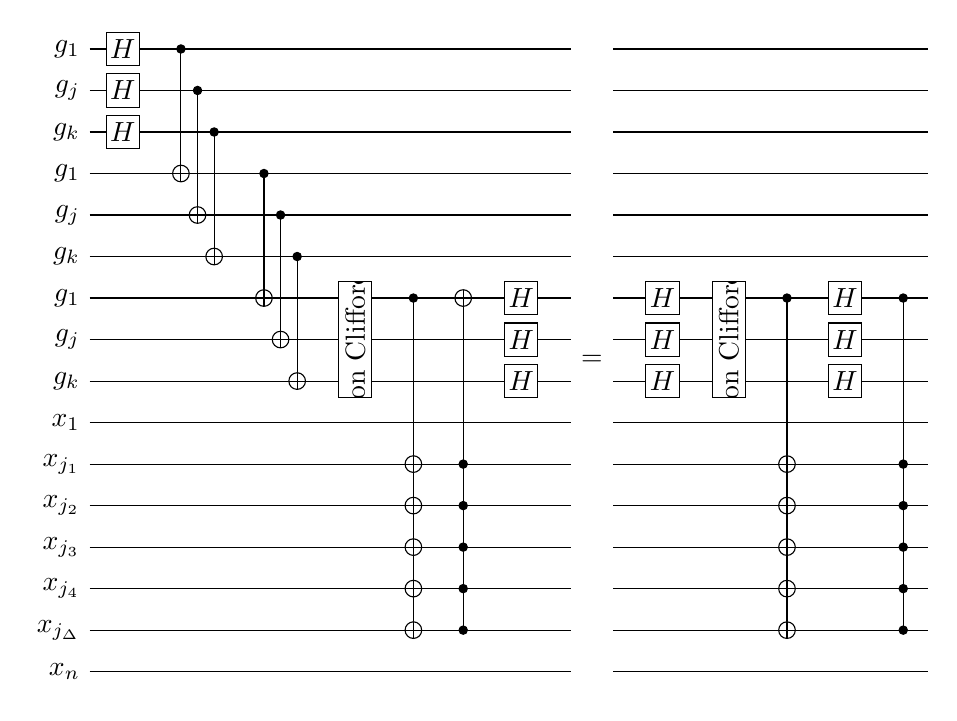
\begin{tikzpicture}[scale=1.000000,x=1pt,y=1pt]
\filldraw[color=white] (0.000000, -7.500000) rectangle (303.000000, 232.500000);
% Drawing wires
% Line 1: aa W g_1
\draw[color=black] (0.000000,225.000000) -- (303.000000,225.000000);
\draw[color=black] (0.000000,225.000000) node[left] {$g_1$};
% Line 2: cc W g_j
\draw[color=black] (0.000000,210.000000) -- (303.000000,210.000000);
\draw[color=black] (0.000000,210.000000) node[left] {$g_j$};
% Line 3: ee W g_k
\draw[color=black] (0.000000,195.000000) -- (303.000000,195.000000);
\draw[color=black] (0.000000,195.000000) node[left] {$g_k$};
% Line 4: aaa W g_1
\draw[color=black] (0.000000,180.000000) -- (303.000000,180.000000);
\draw[color=black] (0.000000,180.000000) node[left] {$g_1$};
% Line 5: ccc W g_j
\draw[color=black] (0.000000,165.000000) -- (303.000000,165.000000);
\draw[color=black] (0.000000,165.000000) node[left] {$g_j$};
% Line 6: eee W g_k
\draw[color=black] (0.000000,150.000000) -- (303.000000,150.000000);
\draw[color=black] (0.000000,150.000000) node[left] {$g_k$};
% Line 7: a W g_1
\draw[color=black] (0.000000,135.000000) -- (303.000000,135.000000);
\draw[color=black] (0.000000,135.000000) node[left] {$g_1$};
% Line 8: c W g_j
\draw[color=black] (0.000000,120.000000) -- (303.000000,120.000000);
\draw[color=black] (0.000000,120.000000) node[left] {$g_j$};
% Line 9: e W g_k
\draw[color=black] (0.000000,105.000000) -- (303.000000,105.000000);
\draw[color=black] (0.000000,105.000000) node[left] {$g_k$};
% Line 11: a2 W x_1
\draw[color=black] (0.000000,90.000000) -- (303.000000,90.000000);
\draw[color=black] (0.000000,90.000000) node[left] {$x_1$};
% Line 12: c2 W x_{j_1}
\draw[color=black] (0.000000,75.000000) -- (303.000000,75.000000);
\draw[color=black] (0.000000,75.000000) node[left] {$x_{j_1}$};
% Line 13: c21 W x_{j_2}
\draw[color=black] (0.000000,60.000000) -- (303.000000,60.000000);
\draw[color=black] (0.000000,60.000000) node[left] {$x_{j_2}$};
% Line 14: c22 W x_{j_3}
\draw[color=black] (0.000000,45.000000) -- (303.000000,45.000000);
\draw[color=black] (0.000000,45.000000) node[left] {$x_{j_3}$};
% Line 15: c23 W x_{j_4}
\draw[color=black] (0.000000,30.000000) -- (303.000000,30.000000);
\draw[color=black] (0.000000,30.000000) node[left] {$x_{j_4}$};
% Line 16: c24 W x_{j_\Delta}
\draw[color=black] (0.000000,15.000000) -- (303.000000,15.000000);
\draw[color=black] (0.000000,15.000000) node[left] {$x_{j_\Delta}$};
% Line 17: e2 W x_n
\draw[color=black] (0.000000,0.000000) -- (303.000000,0.000000);
\draw[color=black] (0.000000,0.000000) node[left] {$x_n$};
% Done with wires; drawing gates
% Line 19: aa H
\begin{scope}
\draw[fill=white] (12.000000, 225.000000) +(-45.000000:8.485281pt and 8.485281pt) -- +(45.000000:8.485281pt and 8.485281pt) -- +(135.000000:8.485281pt and 8.485281pt) -- +(225.000000:8.485281pt and 8.485281pt) -- cycle;
\clip (12.000000, 225.000000) +(-45.000000:8.485281pt and 8.485281pt) -- +(45.000000:8.485281pt and 8.485281pt) -- +(135.000000:8.485281pt and 8.485281pt) -- +(225.000000:8.485281pt and 8.485281pt) -- cycle;
\draw (12.000000, 225.000000) node {$H$};
\end{scope}
% Line 20: cc H
\begin{scope}
\draw[fill=white] (12.000000, 210.000000) +(-45.000000:8.485281pt and 8.485281pt) -- +(45.000000:8.485281pt and 8.485281pt) -- +(135.000000:8.485281pt and 8.485281pt) -- +(225.000000:8.485281pt and 8.485281pt) -- cycle;
\clip (12.000000, 210.000000) +(-45.000000:8.485281pt and 8.485281pt) -- +(45.000000:8.485281pt and 8.485281pt) -- +(135.000000:8.485281pt and 8.485281pt) -- +(225.000000:8.485281pt and 8.485281pt) -- cycle;
\draw (12.000000, 210.000000) node {$H$};
\end{scope}
% Line 21: ee H
\begin{scope}
\draw[fill=white] (12.000000, 195.000000) +(-45.000000:8.485281pt and 8.485281pt) -- +(45.000000:8.485281pt and 8.485281pt) -- +(135.000000:8.485281pt and 8.485281pt) -- +(225.000000:8.485281pt and 8.485281pt) -- cycle;
\clip (12.000000, 195.000000) +(-45.000000:8.485281pt and 8.485281pt) -- +(45.000000:8.485281pt and 8.485281pt) -- +(135.000000:8.485281pt and 8.485281pt) -- +(225.000000:8.485281pt and 8.485281pt) -- cycle;
\draw (12.000000, 195.000000) node {$H$};
\end{scope}
% Line 23: aa +aaa
\draw (33.000000,225.000000) -- (33.000000,180.000000);
\filldraw (33.000000, 225.000000) circle(1.500000pt);
\begin{scope}
\draw[fill=white] (33.000000, 180.000000) circle(3.000000pt);
\clip (33.000000, 180.000000) circle(3.000000pt);
\draw (30.000000, 180.000000) -- (36.000000, 180.000000);
\draw (33.000000, 177.000000) -- (33.000000, 183.000000);
\end{scope}
% Line 24: cc +ccc
\draw (39.000000,210.000000) -- (39.000000,165.000000);
\filldraw (39.000000, 210.000000) circle(1.500000pt);
\begin{scope}
\draw[fill=white] (39.000000, 165.000000) circle(3.000000pt);
\clip (39.000000, 165.000000) circle(3.000000pt);
\draw (36.000000, 165.000000) -- (42.000000, 165.000000);
\draw (39.000000, 162.000000) -- (39.000000, 168.000000);
\end{scope}
% Line 25: ee +eee
\draw (45.000000,195.000000) -- (45.000000,150.000000);
\filldraw (45.000000, 195.000000) circle(1.500000pt);
\begin{scope}
\draw[fill=white] (45.000000, 150.000000) circle(3.000000pt);
\clip (45.000000, 150.000000) circle(3.000000pt);
\draw (42.000000, 150.000000) -- (48.000000, 150.000000);
\draw (45.000000, 147.000000) -- (45.000000, 153.000000);
\end{scope}
% Line 27: aaa +a
\draw (63.000000,180.000000) -- (63.000000,135.000000);
\filldraw (63.000000, 180.000000) circle(1.500000pt);
\begin{scope}
\draw[fill=white] (63.000000, 135.000000) circle(3.000000pt);
\clip (63.000000, 135.000000) circle(3.000000pt);
\draw (60.000000, 135.000000) -- (66.000000, 135.000000);
\draw (63.000000, 132.000000) -- (63.000000, 138.000000);
\end{scope}
% Line 28: ccc +c
\draw (69.000000,165.000000) -- (69.000000,120.000000);
\filldraw (69.000000, 165.000000) circle(1.500000pt);
\begin{scope}
\draw[fill=white] (69.000000, 120.000000) circle(3.000000pt);
\clip (69.000000, 120.000000) circle(3.000000pt);
\draw (66.000000, 120.000000) -- (72.000000, 120.000000);
\draw (69.000000, 117.000000) -- (69.000000, 123.000000);
\end{scope}
% Line 29: eee +e
\draw (75.000000,150.000000) -- (75.000000,105.000000);
\filldraw (75.000000, 150.000000) circle(1.500000pt);
\begin{scope}
\draw[fill=white] (75.000000, 105.000000) circle(3.000000pt);
\clip (75.000000, 105.000000) circle(3.000000pt);
\draw (72.000000, 105.000000) -- (78.000000, 105.000000);
\draw (75.000000, 102.000000) -- (75.000000, 108.000000);
\end{scope}
% Line 31: a c e G \rotatebox{90}{Non Cliffords}
\draw (96.000000,135.000000) -- (96.000000,105.000000);
\begin{scope}
\draw[fill=white] (96.000000, 120.000000) +(-45.000000:8.485281pt and 29.698485pt) -- +(45.000000:8.485281pt and 29.698485pt) -- +(135.000000:8.485281pt and 29.698485pt) -- +(225.000000:8.485281pt and 29.698485pt) -- cycle;
\clip (96.000000, 120.000000) +(-45.000000:8.485281pt and 29.698485pt) -- +(45.000000:8.485281pt and 29.698485pt) -- +(135.000000:8.485281pt and 29.698485pt) -- +(225.000000:8.485281pt and 29.698485pt) -- cycle;
\draw (96.000000, 120.000000) node {\rotatebox{90}{Non Cliffords}};
\end{scope}
% Line 33: a +c2 +c21 +c22 +c23 +c24
\draw (117.000000,135.000000) -- (117.000000,15.000000);
\filldraw (117.000000, 135.000000) circle(1.500000pt);
\begin{scope}
\draw[fill=white] (117.000000, 75.000000) circle(3.000000pt);
\clip (117.000000, 75.000000) circle(3.000000pt);
\draw (114.000000, 75.000000) -- (120.000000, 75.000000);
\draw (117.000000, 72.000000) -- (117.000000, 78.000000);
\end{scope}
\begin{scope}
\draw[fill=white] (117.000000, 60.000000) circle(3.000000pt);
\clip (117.000000, 60.000000) circle(3.000000pt);
\draw (114.000000, 60.000000) -- (120.000000, 60.000000);
\draw (117.000000, 57.000000) -- (117.000000, 63.000000);
\end{scope}
\begin{scope}
\draw[fill=white] (117.000000, 45.000000) circle(3.000000pt);
\clip (117.000000, 45.000000) circle(3.000000pt);
\draw (114.000000, 45.000000) -- (120.000000, 45.000000);
\draw (117.000000, 42.000000) -- (117.000000, 48.000000);
\end{scope}
\begin{scope}
\draw[fill=white] (117.000000, 30.000000) circle(3.000000pt);
\clip (117.000000, 30.000000) circle(3.000000pt);
\draw (114.000000, 30.000000) -- (120.000000, 30.000000);
\draw (117.000000, 27.000000) -- (117.000000, 33.000000);
\end{scope}
\begin{scope}
\draw[fill=white] (117.000000, 15.000000) circle(3.000000pt);
\clip (117.000000, 15.000000) circle(3.000000pt);
\draw (114.000000, 15.000000) -- (120.000000, 15.000000);
\draw (117.000000, 12.000000) -- (117.000000, 18.000000);
\end{scope}
% Line 34: +a c2 c21 c22 c23 c24
\draw (135.000000,135.000000) -- (135.000000,15.000000);
\begin{scope}
\draw[fill=white] (135.000000, 135.000000) circle(3.000000pt);
\clip (135.000000, 135.000000) circle(3.000000pt);
\draw (132.000000, 135.000000) -- (138.000000, 135.000000);
\draw (135.000000, 132.000000) -- (135.000000, 138.000000);
\end{scope}
\filldraw (135.000000, 75.000000) circle(1.500000pt);
\filldraw (135.000000, 60.000000) circle(1.500000pt);
\filldraw (135.000000, 45.000000) circle(1.500000pt);
\filldraw (135.000000, 30.000000) circle(1.500000pt);
\filldraw (135.000000, 15.000000) circle(1.500000pt);
% Line 36: a H
\begin{scope}
\draw[fill=white] (156.000000, 135.000000) +(-45.000000:8.485281pt and 8.485281pt) -- +(45.000000:8.485281pt and 8.485281pt) -- +(135.000000:8.485281pt and 8.485281pt) -- +(225.000000:8.485281pt and 8.485281pt) -- cycle;
\clip (156.000000, 135.000000) +(-45.000000:8.485281pt and 8.485281pt) -- +(45.000000:8.485281pt and 8.485281pt) -- +(135.000000:8.485281pt and 8.485281pt) -- +(225.000000:8.485281pt and 8.485281pt) -- cycle;
\draw (156.000000, 135.000000) node {$H$};
\end{scope}
% Line 37: c H
\begin{scope}
\draw[fill=white] (156.000000, 120.000000) +(-45.000000:8.485281pt and 8.485281pt) -- +(45.000000:8.485281pt and 8.485281pt) -- +(135.000000:8.485281pt and 8.485281pt) -- +(225.000000:8.485281pt and 8.485281pt) -- cycle;
\clip (156.000000, 120.000000) +(-45.000000:8.485281pt and 8.485281pt) -- +(45.000000:8.485281pt and 8.485281pt) -- +(135.000000:8.485281pt and 8.485281pt) -- +(225.000000:8.485281pt and 8.485281pt) -- cycle;
\draw (156.000000, 120.000000) node {$H$};
\end{scope}
% Line 38: e H
\begin{scope}
\draw[fill=white] (156.000000, 105.000000) +(-45.000000:8.485281pt and 8.485281pt) -- +(45.000000:8.485281pt and 8.485281pt) -- +(135.000000:8.485281pt and 8.485281pt) -- +(225.000000:8.485281pt and 8.485281pt) -- cycle;
\clip (156.000000, 105.000000) +(-45.000000:8.485281pt and 8.485281pt) -- +(45.000000:8.485281pt and 8.485281pt) -- +(135.000000:8.485281pt and 8.485281pt) -- +(225.000000:8.485281pt and 8.485281pt) -- cycle;
\draw (156.000000, 105.000000) node {$H$};
\end{scope}
% Line 40: =
\draw[fill=white,color=white] (174.000000, -6.000000) rectangle (189.000000, 231.000000);
\draw (181.500000, 112.500000) node {$=$};
% Line 41: a H
\begin{scope}
\draw[fill=white] (207.000000, 135.000000) +(-45.000000:8.485281pt and 8.485281pt) -- +(45.000000:8.485281pt and 8.485281pt) -- +(135.000000:8.485281pt and 8.485281pt) -- +(225.000000:8.485281pt and 8.485281pt) -- cycle;
\clip (207.000000, 135.000000) +(-45.000000:8.485281pt and 8.485281pt) -- +(45.000000:8.485281pt and 8.485281pt) -- +(135.000000:8.485281pt and 8.485281pt) -- +(225.000000:8.485281pt and 8.485281pt) -- cycle;
\draw (207.000000, 135.000000) node {$H$};
\end{scope}
% Line 42: c H
\begin{scope}
\draw[fill=white] (207.000000, 120.000000) +(-45.000000:8.485281pt and 8.485281pt) -- +(45.000000:8.485281pt and 8.485281pt) -- +(135.000000:8.485281pt and 8.485281pt) -- +(225.000000:8.485281pt and 8.485281pt) -- cycle;
\clip (207.000000, 120.000000) +(-45.000000:8.485281pt and 8.485281pt) -- +(45.000000:8.485281pt and 8.485281pt) -- +(135.000000:8.485281pt and 8.485281pt) -- +(225.000000:8.485281pt and 8.485281pt) -- cycle;
\draw (207.000000, 120.000000) node {$H$};
\end{scope}
% Line 43: e H
\begin{scope}
\draw[fill=white] (207.000000, 105.000000) +(-45.000000:8.485281pt and 8.485281pt) -- +(45.000000:8.485281pt and 8.485281pt) -- +(135.000000:8.485281pt and 8.485281pt) -- +(225.000000:8.485281pt and 8.485281pt) -- cycle;
\clip (207.000000, 105.000000) +(-45.000000:8.485281pt and 8.485281pt) -- +(45.000000:8.485281pt and 8.485281pt) -- +(135.000000:8.485281pt and 8.485281pt) -- +(225.000000:8.485281pt and 8.485281pt) -- cycle;
\draw (207.000000, 105.000000) node {$H$};
\end{scope}
% Line 44: a c e G \rotatebox{90}{Non Cliffords}
\draw (231.000000,135.000000) -- (231.000000,105.000000);
\begin{scope}
\draw[fill=white] (231.000000, 120.000000) +(-45.000000:8.485281pt and 29.698485pt) -- +(45.000000:8.485281pt and 29.698485pt) -- +(135.000000:8.485281pt and 29.698485pt) -- +(225.000000:8.485281pt and 29.698485pt) -- cycle;
\clip (231.000000, 120.000000) +(-45.000000:8.485281pt and 29.698485pt) -- +(45.000000:8.485281pt and 29.698485pt) -- +(135.000000:8.485281pt and 29.698485pt) -- +(225.000000:8.485281pt and 29.698485pt) -- cycle;
\draw (231.000000, 120.000000) node {\rotatebox{90}{Non Cliffords}};
\end{scope}
% Line 45: a +c2 +c21 +c22 +c23 +c24
\draw (252.000000,135.000000) -- (252.000000,15.000000);
\filldraw (252.000000, 135.000000) circle(1.500000pt);
\begin{scope}
\draw[fill=white] (252.000000, 75.000000) circle(3.000000pt);
\clip (252.000000, 75.000000) circle(3.000000pt);
\draw (249.000000, 75.000000) -- (255.000000, 75.000000);
\draw (252.000000, 72.000000) -- (252.000000, 78.000000);
\end{scope}
\begin{scope}
\draw[fill=white] (252.000000, 60.000000) circle(3.000000pt);
\clip (252.000000, 60.000000) circle(3.000000pt);
\draw (249.000000, 60.000000) -- (255.000000, 60.000000);
\draw (252.000000, 57.000000) -- (252.000000, 63.000000);
\end{scope}
\begin{scope}
\draw[fill=white] (252.000000, 45.000000) circle(3.000000pt);
\clip (252.000000, 45.000000) circle(3.000000pt);
\draw (249.000000, 45.000000) -- (255.000000, 45.000000);
\draw (252.000000, 42.000000) -- (252.000000, 48.000000);
\end{scope}
\begin{scope}
\draw[fill=white] (252.000000, 30.000000) circle(3.000000pt);
\clip (252.000000, 30.000000) circle(3.000000pt);
\draw (249.000000, 30.000000) -- (255.000000, 30.000000);
\draw (252.000000, 27.000000) -- (252.000000, 33.000000);
\end{scope}
\begin{scope}
\draw[fill=white] (252.000000, 15.000000) circle(3.000000pt);
\clip (252.000000, 15.000000) circle(3.000000pt);
\draw (249.000000, 15.000000) -- (255.000000, 15.000000);
\draw (252.000000, 12.000000) -- (252.000000, 18.000000);
\end{scope}
% Line 47: a H
\begin{scope}
\draw[fill=white] (273.000000, 135.000000) +(-45.000000:8.485281pt and 8.485281pt) -- +(45.000000:8.485281pt and 8.485281pt) -- +(135.000000:8.485281pt and 8.485281pt) -- +(225.000000:8.485281pt and 8.485281pt) -- cycle;
\clip (273.000000, 135.000000) +(-45.000000:8.485281pt and 8.485281pt) -- +(45.000000:8.485281pt and 8.485281pt) -- +(135.000000:8.485281pt and 8.485281pt) -- +(225.000000:8.485281pt and 8.485281pt) -- cycle;
\draw (273.000000, 135.000000) node {$H$};
\end{scope}
% Line 48: c H
\begin{scope}
\draw[fill=white] (273.000000, 120.000000) +(-45.000000:8.485281pt and 8.485281pt) -- +(45.000000:8.485281pt and 8.485281pt) -- +(135.000000:8.485281pt and 8.485281pt) -- +(225.000000:8.485281pt and 8.485281pt) -- cycle;
\clip (273.000000, 120.000000) +(-45.000000:8.485281pt and 8.485281pt) -- +(45.000000:8.485281pt and 8.485281pt) -- +(135.000000:8.485281pt and 8.485281pt) -- +(225.000000:8.485281pt and 8.485281pt) -- cycle;
\draw (273.000000, 120.000000) node {$H$};
\end{scope}
% Line 49: e H
\begin{scope}
\draw[fill=white] (273.000000, 105.000000) +(-45.000000:8.485281pt and 8.485281pt) -- +(45.000000:8.485281pt and 8.485281pt) -- +(135.000000:8.485281pt and 8.485281pt) -- +(225.000000:8.485281pt and 8.485281pt) -- cycle;
\clip (273.000000, 105.000000) +(-45.000000:8.485281pt and 8.485281pt) -- +(45.000000:8.485281pt and 8.485281pt) -- +(135.000000:8.485281pt and 8.485281pt) -- +(225.000000:8.485281pt and 8.485281pt) -- cycle;
\draw (273.000000, 105.000000) node {$H$};
\end{scope}
% Line 51: a c2 c21 c22 c23 c24
\draw (294.000000,135.000000) -- (294.000000,15.000000);
\filldraw (294.000000, 135.000000) circle(1.500000pt);
\filldraw (294.000000, 75.000000) circle(1.500000pt);
\filldraw (294.000000, 60.000000) circle(1.500000pt);
\filldraw (294.000000, 45.000000) circle(1.500000pt);
\filldraw (294.000000, 30.000000) circle(1.500000pt);
\filldraw (294.000000, 15.000000) circle(1.500000pt);
% Done with gates; drawing ending labels
% Done with ending labels; drawing cut lines and comments
% Done with comments
\end{tikzpicture}

\begin{figure}[h]
  \begin{subfigure}[b]{0.45\textwidth}
    \begin{claim}
      The state:
      \begin{equation*}
        \begin{split}
          \sum_{z \in C_{Z}^{\perp}}  \exp \Big(  & -  2 \cdot \pi/4 \sum_{g ,h
            \in \text{ gen } C_{Z}^{\perp}} \hat{X}_{g}\hat{X}_{h}|g\cdot h| \\
            & +  4 \cdot i\pi/4 \sum_{g,h \in \text{ gen } C_{Z}^{\perp}}
          \hat{X}_{g}\hat{X}_{h}\hat{X}_{l}|g\cdot h \cdot l|  \Big) \ket{z}
        \end{split}
      \end{equation*}
      Can be computed such that any
    \end{claim}
  \end{subfigure}
  \begin{subfigure}[b]{0.05\textwidth}
    \
  \end{subfigure}
  \begin{subfigure}[b]{0.45\textwidth}
  \end{subfigure}
\end{figure}

\begin{proof}
  Denote by $U_{v}$ the gate which turn on all the generators supported on $v$.
  As any of them is just of a code word of $C_{A}\otimes C_{B}$, namely turning
  on generator require touching at most constant number of qubits combing
\end{proof}

\begin{claim}
  \label{claim:lowlightcone}
  The state $\left(M_{2}^{\dagger}\otimes I\right)\ket{ C_{Z}^{\perp} +
  \Lambda   }\ket{0}$ can be computed, such that the light cone depth of any
  non-clifford gate is bounded by constant.
\end{claim}
\begin{proof}
  \begin{align*}
    \left( I \otimes H_{X} \right) CX_{n\rightarrow n} \left(E \otimes E
    \right) \ \ I \otimes L[M_{2}^{\dagger}] \ \ & \prod_{\substack{ J\in \{
    \text{ gen }\Lambda,\\ \text{ gen } C_{Z}^{\perp} \}}} \prod_{g \in J}
    \left(
    I +  X_{L[g]} \right) && \ket{0} \ket{0} \\
    = \left( I \otimes H_{X}   \right) CX_{n\rightarrow n} & \sum_{\substack{ z
    \in C_{Z}^\perp \\  x\in \Lambda}}  e^{\varphi(z)} && \ket{x}\ket{z} \\
    = & \sum_{\substack{ z \in C_{Z}^\perp \\  x\in \Lambda}}   e^{\varphi(z)}
    && \ket{x+z}\ket{0} \\
    = & \sum_{\substack{ z \in C_{Z}^\perp \\  x\in \Lambda}}
    \left(M_{2}^{\dagger}\otimes I\right) && \ket{x+z}\ket{0} \\
    = & \left(M_{2}^{\dagger}\otimes I\right) && \ket{ C_{Z}^{\perp} +
    \Lambda   }\ket{0}
  \end{align*}
\end{proof}
Denote by $p \in [0,1]$ the error rate of input magic states, and let $\ket{A}$
be an ancilla initialized to a one-qubit magic state. This $\ket{A}$ can be
used to compute the $T$ gate, with a probability of $Z$ error occurring with a
probability of $p$ \cite{bravyi2012magic}.
\begin{claim}
  There are constant numbers $\zeta_{\Delta},\xi_{\Delta}$, and a circuit
  $\mathcal{C}$ such that:
  \begin{enumerate}
    \item In the no-noise setting, The circuit compute the state
      \begin{equation*}
        \begin{split}
          \mathcal{C} \ket{0}^{\Theta(n)} \otimes \ket{A}^{\Theta(n)}
          \rightarrow  \prod_{g \in \text{ gen }\Lambda} T_{g} \ket{
            C_{Z}^{\perp} +
          \Lambda   }
        \end{split}
      \end{equation*}
    \item Otherwise, the circuit computes the state
      \begin{equation*}
        \begin{split}
          \mathcal{C} \ket{0}^{\Theta(n)} \otimes \ket{A}^{\Theta(n)}
          \rightarrow Z^{e} \ \ \ \prod_{g \in \text{ gen } \Lambda} T_{g} \ket{
          C_{Z}^{\perp} +  \Lambda   }
        \end{split}
      \end{equation*}
      , where the probability that $e_{i} = 1$ is less than $\zeta_{\Delta}
      \cdot  p$. Additionally, for any $i$, there are at most $\xi_{\Delta}$
      indices
      $j$ such that $e_{i}$ and $e_{j}$ are dependent.
  \end{enumerate}
\end{claim}

\begin{proof}
  Concatinate the $T^{n} \otimes I $ with the gate in \Cref{claim:lowlightcone}.
\end{proof}

\begin{claim}
  For any $\alpha \in (0,1)$ the probability that
  $|e|>(1+\alpha)p\zeta_{\Delta}$ is less than:
  \begin{equation*}
    \begin{split}
      \prb{ |e| > (1+\alpha) \expp{|e|} } < \frac{1\cdot
      \xi_{\Delta}n}{\alpha^{2}\zeta_{\Delta}^{2}p^{2}n^{2}} = o\left( 1/n
      \right)
    \end{split}
  \end{equation*}
\end{claim}
\begin{proof}
  By the Chebyshev inequality, notice that the number for which
  $\expp{e_{i}e_{j}}-\expp{e_{i}}\expp{e_{j}} \neq 0$ is less than
  $\xi_{\Delta}n$.
\end{proof}

\begin{definition}
  We will said that a decoder $\mathcal{D}$ for the good qunatum LDPC code is
  an good-local decoder if
  \begin{enumerate}
    \item There is a treashold $\mu n$ such that if the error size is less than
      $|e| < \mu n$ then $\mathcal{D}$ correct $e$ in constant number of rounds.
      With probability $ 1 - o(1/n)$.
    \item In any rounds $\mathcal{D}$ performs at most $O(n)$ work (depth
      $\times$ width).
    \item The above is true in operation-noisy settings, where there is a
      probability of $p$ for an error to occur after acting on a qubit.
      ($\star$)
  \end{enumerate}
  $\star$ The motivation for this is that if the decoder does not act on the
  qubit, then it also does not apply a $T$ gate on it. Therefore, in the
  distillation setting, there is zero chance for an error to occur.
\end{definition}

\begin{claim}
  Suppose there is a good local decoder $\mathcal{D}$ for the good qLDPC code.
  Then, there exists $p_{0}$ such that for any sufficiently large $n$, there is
  a distillation protocol that, given $\Theta(n)$ magic states at an error rate
  $p<p_{0}$, successfully distills $\Theta(n)$ perfect magic states with a
  probability of $1 - o(1/n)$. Furthermore, the protocol's space and time
  complexity (both quantum and classical) are $\Theta(n)$ and $\Theta(n^{2})$,
  respectively.
\end{claim}

\ifdefined\MORE

\begin{figure}[h]
  \begin{subfigure}[t]{0.65\textwidth}
    \begin{definition}
      Let $M \in \mathbb{F}_{2}^{k \times n }$ upper triangular matrix such
      that~$k~<~n$. We say that $M$ has the $1$-stairs property if $M_{ij}=1$
      any
      $j<i$.
    \end{definition}
    \begin{claim}
      \label{claim:stair}
      Any $M \in \mathbb{F}_{2}^{k \times n }$ upper triangular matrix can be
      turn into upper triangular matrix that has the $1$-stairs property by
      elementary operation.
    \end{claim}

  \end{subfigure}
  \begin{subfigure}[t]{0.05\textwidth}
    \
  \end{subfigure}
  \begin{subfigure}[t]{0.25\textwidth}

    \begin{equation*}
      \begin{split}
        \begin{bmatrix}
          1 & 1 & 1 &1 &1 &\cdot & \cdot & \cdot & \cdot & \cdot \\
          0 & 1 & 1 &1 &1 &\cdot & \cdot & \cdot & \cdot & \cdot \\
          0 & 0 & 1 &1 &1 &\cdot & \cdot & \cdot & \cdot & \cdot \\
          0 & 0 & 0 &1 &1 &\cdot & \cdot & \cdot & \cdot & \cdot \\
          0 & 0 & 0 &0 &1 &\cdot & \cdot & \cdot & \cdot & \cdot
        \end{bmatrix}
      \end{split}
    \end{equation*}

  \end{subfigure}
\end{figure}
\begin{proof}
  Consider the following algorithm: Let $M$ be our initial matrix. We iterate
  over the rows from left to right. In the $i$th iteration, we check for any row
  $j<i$ if $M_{ji} = 1$. If not, we set $M$ to be the matrix obtained by adding
  the $i$th row to the $j$th row. Since $M$ is an upper triangular matrix,
  adding the $i$th row does not change any entry $M_{js}$ for $s<i$. Therefore,
  the obtained matrix is still an upper triangular matrix and the entries at
  $M_{js}$ for $j,s < i$ remain the same, namely $1$ if and only if $j\le s$.

  Continuing with the process eventually yields, after $k$ iterations, a matrix
  with the $1$-stair property.
\end{proof}

\begin{claim}
  The logical operator $CX_{g}$ relative the code $C_{Z}^{\perp}$ can be
  implement such it acts on constant number of qubits. \textbf{Notice,}
  implementation of the gate $CX_{g}$ relative to $C_{Z}^{\perp}$ might
  incorrect for computing $CX_{g}$ relative to $C_{X}$.
\end{claim}

\begin{definition}[Source of $g \in C_{Z}^{\perp}$.]
  Let $C$ be the quantum Tanner code, and let $g$ be a generator of
  $C_{Z}^{\perp}$. The vertex $v$ will be called the source of $g$. If $g$ is a
  codeword of the tensor code $C_{A}\otimes C_{B}$, it can be viewed locally on
  $g$.
\end{definition}

\begin{figure}[h]
  \begin{subfigure}{0.5\textwidth}
    \begin{proof}
      Let $g$ be a generator of $C_{Z}^{\perp}$. As the generators of
      $C_{Z}^\perp$ are defined to be the set of codewords of some 'small code'
      ($C_{0}$) over the local view of the vertices in a $\Delta$-regular
      graph, it
      holds that first, there is a vertex $v$ on which $g$ is supported. Second,
      only the generators supported by $v$'s neighbors have a non-vanishing
      overlap
      with $g$.

      Let $g$ be a generator of $C_{Z}^{\perp}$ and denote by $v$ the source of
      $g$. First, we will prove that there exist $\xi_{1}, \xi_{2}, \xi_{3} \in
      \mathbb{F}_{2}^{N}$ such that each $\xi_{i}$ has a weight of at most
      $\frac{1}{2} \Delta$, $\xi_{i} \cdot g = 1$, and for any other generator
      $h
      \neq g$ in $C_{Z}^{\perp}$, there is at least one $i$ such that $\xi_{i}
      \cdot
      h = 0$.

      Let $B_1, B_2, B_3$ be subsets of $[\Delta]$ such that $|B_i| =
      \frac{2}{3}\Delta$ and $B_1 \cap B_2 \cap B_3 = \emptyset$. Now, define
      $\xi_i$ to be the vector supported only on $B_i$ and satisfies $\xi_i
      \cdot g
      = 1$. For any other generator $h$ such that $v$ is its source, and also
      $h|_{B_{i}} \neq g|_{B_{i}}$, we have $\xi_i \cdot h = 0$. Notice that for
      every $h \neq g$, there must be at least one $B_{i}$ for which $g|_{B_{i}}
      \neq h|_{B_{i}}$. Each $x_{i}$ is a solution for a linear system with (at
      most) $\rho\Delta$ equations and $\frac{1}{2} \Delta$ bits. So, if $1/2 >
      \rho$, then there is a solution for each equations system.

      Clearly, for any generator $h$ such $v$ is it's source there are not
      $i$'s such $\xi_{i}h = 1$. It's left to show for remian generators.

    \end{proof}
  \end{subfigure}
  \begin{subfigure}{0.05\textwidth}
    \
  \end{subfigure}
  \begin{subfigure}[t]{0.4\textwidth}
    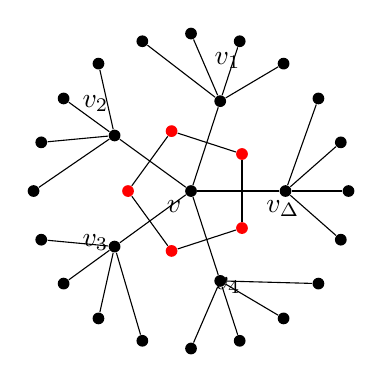
\begin{tikzpicture}
      \begin{scope}[shift={({0},{-2})}]
        \foreach \i in {1,...,5}
        \node[circle, fill=black, inner sep=1.5pt] (\i) at (72*\i:1.2) {};
        \foreach \i in {1,...,5}
        \node[circle, fill=red, inner sep=1.5pt] (\i\i) at (72*\i-36:0.8) {};

        \foreach \i in {1,...,5}
        \foreach \j in {1,...,4}
        \node[circle, fill=black, inner sep=1.5pt] (5*\i+\j) at
        (72*\i+18*\j-36:2) {};
        \node[circle, fill=black, inner sep=1.5pt] (0) at (0,0) {};
        % edges
        \foreach \i in {1,...,5}
        \draw (\i) -- (0);
        \foreach \i[evaluate=\i as \m using int(\i+1)] in {1,...,4}
        \draw (\i\i) -- (\m\m);
        \draw (55) -- (11);
        \foreach \i in {1,...,5}
        \foreach \j in {1,...,4}
        \draw (\i) -- (5*\i+\j);
        % labels
        \foreach \i in {1,...,4}
        \node[above] at (72*\i:1.5) {$v_{\i}$};
        \node[anchor=north east] at (72*5:1.5) {$v_{\Delta}$};
        \node[anchor=north east] at (0,0) {$v$};
      \end{scope}
    \end{tikzpicture}
  \end{subfigure}
\end{figure}

\begin{claim}
  Let $Q =(C_{X},C_{Z})$ a good qLDPC CSS code. Then for any $g$ generator in
  $C_{Z}^{\perp}$ there is a logical gate compute $CX_{g}$ acting on at most
  $O(1)$ qubits.
\end{claim}
\begin{proof}
  Recall that the generator matrix of $C_{Z}^\perp$ is the parity check matrix
  of $C_{Z}$. So we are looking for $\xi$ such that:
  \begin{equation*}
    \begin{split}
      H_{Z}
      \begin{bmatrix}
        | \\
        | \\
        \xi \\
        | \\
        |
      \end{bmatrix} =
      \begin{bmatrix}
        1 \\
        0 \\
        0 \\
        0 \\
        0
      \end{bmatrix}
    \end{split}
  \end{equation*}
  Assume that there is solution $\xi$ for the equations system. If $H_{z}$ is a
  parity check matrix of ltc code then $d(\xi,C_{Z}) = O(1)$ so we could picck
  some $z+\xi$ such that $z\in C_{Z}$ and having a solution that it's weight is
  $O(1)$.   %, then any $z + \xi$  where $z \in C_{Z}$ is also a solution.
  % \prod_{z_{r_i^{\prime}}}
  \begin{equation*}
    \begin{split}
      \sum_{r_{i},l_{j}}\ket{z_{r_i}}\ket{z_{l_j}} & =
      \sum_{z_{r_i^{\prime}}}\sum_{r_{i},l_{j}}\ket{z_{r_i}}\ket{z_{l_j}} \ket{
        0 +
      \xi[z_{r_{i^{\prime}}}]\cdot z_{r_{i}} } \sum_{z_{l_j^{\prime}}} \\
      x &
    \end{split}
  \end{equation*}

\end{proof}

\newcommand{\hashcode}{ checks-hashed }

\begin{definition}
  Let $\{h_{i} \}_{1}^{t}$ be the checks of $\Delta$-length code $C_{0}$. We
  say that $i$th bit and the $j$th bit collide if there a check $h$ such that
  $h_{i}=h_{j}=1$. We say that a $C_{0}$ is a \hashcode if:
  \begin{equation*}
    \begin{split}
      \prbm{ i,j \text{ collide  }  }{ i, j \sim [\Delta]^{2} } <
      \frac{1}{2\Delta}
    \end{split}
  \end{equation*}
\end{definition}

\begin{claim}
  Suppose that $C_{0}^{\perp}$ is a \hashcode. Then $\left( C_{0}^{\otimes m}
  \right)^{\perp}$ is also a \hashcode.
\end{claim}
\begin{proof}

  \begin{equation*}
    \begin{split}
      \prbm{X^{(m)}_{u,v}}{u,v\sim [n]^{2}} \le & \prbm{X^{(1)}_{u,v}}{u,v\sim
      [\Delta]^{2}} \cdot \prbm{X^{(m-1)}_{u,v} }{u,v\sim [n/\Delta]^{2}} \\
      \le & \frac{1}{2\Delta} \cdot \left( \frac{1}{2\Delta} \right)^{m-1} =
      \left( \frac{1}{2\Delta} \right)^{m}
    \end{split}
  \end{equation*}
\end{proof}

Consider the following decoder, we flip a bit if flipping it decrease the
syndrome. Now observers that if a non faulty bit $i$ has been flip then it
means that there is at least one faulty bit $j$ in the error $e$ that $i,j$
collide. Similarly if a faulty bit $i$ hasn't been flip then it means that
there is another faulty bit $j$ that collide with him. In overall we conclude
that the total number of incorrect flips made by the decoder is at most the
number of collisions.

\begin{equation*}
  \begin{split}
    \expp{\sum_{v \in e} \sum_{u \in [n]} X_{v,u}} \le |e|\cdot n \cdot \left(
    \frac{1}{2\Delta} \right)^{m} = \frac{|e|}{2^{m}}
  \end{split}
\end{equation*}

Now we are going to add a random error at weight $\frac{|e|}{2^{m}}$ to ensure
that in the next iteration the $\frac{|e|}{2^{m-1}}$ error will distributed
uniformly. Repeating for $\log_{2^{m-1}}$ rounds correct the error. (not
exactly there is an error in each round that should be handled).

\ctt{ We flip in over all $|e| \sum \frac{1}{2^{i}}  < 2|e| $ bits, so we would
like to have $|e| \le d/4 $.}

\ctt{ Yet we can do better, if $ e = z + \tilde{e}$ where $z$ commute with all
our generators. }

\ctt{ And if it anticommute with only $l$ of them, then we have only $l$
errors. }

\begin{equation*}
  \begin{split}
    \Delta^{m}\le 1/p^{2}_{0} & \rightarrow \alpha \cdot 1/p^{2}_{0} ,
    \frac{m}{2^{m}} \log \Delta
  \end{split}
\end{equation*}

\begin{claim}
  Let $H$ be a $|V|\times r$ binary parity check matrix of $\tilde{C}$. Also,
  let $G$ be a $\Delta$-regular graph. A bit assignment over $G$ edges $x$ will
  be said to be $\tilde{C}$-vertices-respect if the vector $z(x) \in
  \mathbb{F}_{2}^{|V|}$ which is defined as:
  \begin{equation*}
    z(x)_{v} =
    \begin{cases}
      1 & v \text{ sees at least one } 1\\
      0 & \text{otherwise}
    \end{cases}
  \end{equation*}
  is a codeword of $\tilde{C}$. Let $\Lambda$ be the set of all
  $\tilde{C}$-vertices-respect assignments. Then $|\Lambda| >
  (1-\varepsilon)2^{\rho |V|}$.
\end{claim}

\begin{proof}
  Any $x \in \Lambda$ is a solution for the following system of equations:
  \begin{equation*}
    \begin{split}
      z_{v} &= 1 + \prod_{ e \in v }{ \left( 1 - x_{e} \right) } \\
      Hz &= 0
    \end{split}
  \end{equation*}
\end{proof}

\begin{claim}
  Assume that $C_{0}$ is a $\Delta$-length code such that for any two
  non-trival codewords $c,c^{\prime}\in C_{0}$ we have that $c\cdot
  c^{\prime}=1$, and denote by $C = \mathcal{T}(G,C_{0})$. And let $\Lambda$ be
  a the set of all $\tilde{C}$-vertices-respect assignments where $\tilde{C}$
  satisfies relation $R$. Then also $C \cap \Lambda$ satisfies $R$.
\end{claim}

Let $\ket{f}$ be a codeword in $C_{X}$, and let $X_{g}$ be the indicator that
equals $1$ if $f$ has support on $X_{g}$, and $0$ otherwise. Observes that
applying $T^{\otimes}$ on $\ket{f}$ yilds the state:
\begin{equation*}
  \begin{split}
    T^{\otimes n}\ket{f} & =  T^{\otimes n}\ket{\sum_{g} X_{g}g } = \exp \Big(
      i\pi/4 \sum_{g} X_{g}|g|  -  2 \cdot i \pi/4 \sum_{g,h} X_{g}X_{h}|g\cdot
      h| \\
      & +  4 \cdot i\pi/4 \sum_{g,h} X_{g}X_{h}X_{l}|g\cdot h \cdot l| -   8
    \cdot i\pi/4 \cdot \text{ integers } \Big) \ket{f} \\
    & = \exp \Big( i\pi/4 \sum_{g} X_{g}|g|  -  2 \cdot \pi/4 \sum_{g,h}
      X_{g}X_{h}|g\cdot h| +  4 \cdot i\pi/4 \sum_{g,h} X_{g}X_{h}X_{l}|g\cdot h
    \cdot l| \Big) \ket{f}
  \end{split}
\end{equation*}

\section{Many to One.}
Assume that $f$ is supported on exactly one generator. Then we have that
$T^{\otimes n}\ket{f}  = e^{i\pi|g|/4}\ket{f}$ Therefore, if $|g| = 4k+1$ then
we are done.

\section{Using Quntum Error Correction Codes.}

Now assume that the code $C_{X}$ is the quantum Tanner code, denote by $G,A,B$
the group and the two generator sets that are used for constructing the square
complex.

\begin{claim}
  Consider $g,h$ that are supported on the same $v\in V$. We will call such a
  pair a source-sharing pair. Suppose that for any we have that $|g \cdot h|$ is
  even. Then there is a Clifford gate that computes $\ket{f} \mapsto \exp \Big(
  -  i\pi \sum_{g,h \text{ source-sharing }} X_{g}X_{h}|g\cdot h|  \Big) \ket{f}
  $.
\end{claim}
%
%%\begin{claim}
%%  \label{claim:phase}
%%  The gate $\ket{f} \mapsto \exp \Big(   i\pi \sum_{g,h}
% X_{g}X_{h}X_{l}|g\cdot h \cdot l| \Big) \ket{f} $ is in the Clifford group.
%%\end{claim}
%%
%%\begin{proof}
%%  Just decode $f$ and apply \textbf{CCZ} between any triple of qubits
% corresponding to the generators $g,h,l$ such that $g \cdot h \cdot l=_{2} 1$.
% Then encode the state again. Observes that \textbf{CCZ} is a Clifford gate,
% and by the fact that the code is a CSS code then the decoder and the encoder
% are both in the Clifford.
%%\end{proof}
%%
%
%
%\section{Fail Attempt.}
%
%
%In addition, let us assume the existence of $d \in G$ such that $d$ is
% non-identity and commutes with any element in $A \cup B$. Then, observe that
% multiplying by $d$ preserves adjacency on the complex. Namely, if $\{u,v\}
% \in E$ then also $\{du, dv\} \in E$.
%
%Consider $\ket{f}$ such that if $X_g$ is not zero, and $g$ is associated with
% a local codeword $c \in C_A \otimes C_B$ on vertex $v$, then the generator
% associated with the local codeword $c$ on vertex $d \cdot v$ also supports
% $f$, denoted by $g'$. Thus, the exponent above becomes:
%
%\begin{equation*}
%  \begin{split}
%    & = \exp \Big( i\pi/4 \sum_{g} X_{g}|g|  -  2 \cdot \pi/4 \sum_{g,h \in G
% /a} X_{g}X_{h}|g\cdot h| + X_{g^{\prime}}X_{h^{\prime}}|g\cdot h |  \\
%    & +  4 \cdot i\pi/4 \sum_{g,h \in G/a} X_{g}X_{h}X_{l}|g\cdot h \cdot l| +
% X_{g^{\prime}}X_{h^{\prime}}X_{l^{\prime}}|g\cdot h \cdot l| \Big) \ket{f} \\
%    & = \exp \Big( i\pi/4 \sum_{g} X_{g}|g|  -  2 \cdot 2 \cdot \pi/4
% \sum_{g,h \in G/a} X_{g}X_{h}|g\cdot h| +  2 \cdot 4 \cdot i\pi/4 \sum_{g,h
% \in G/a} X_{g}X_{h}X_{l}|g\cdot h \cdot l| \Big) \ket{f} \\
%    & = \exp \Big( i\pi/4 \sum_{g} X_{g}|g|  -  i\pi \sum_{g,h \in G/a}
% X_{g}X_{h}|g\cdot h|  \Big) \ket{f}
%  \end{split}
%\end{equation*}
%
%\begin{figure}
%  \centering
%  \scalebox{0.1}{
%    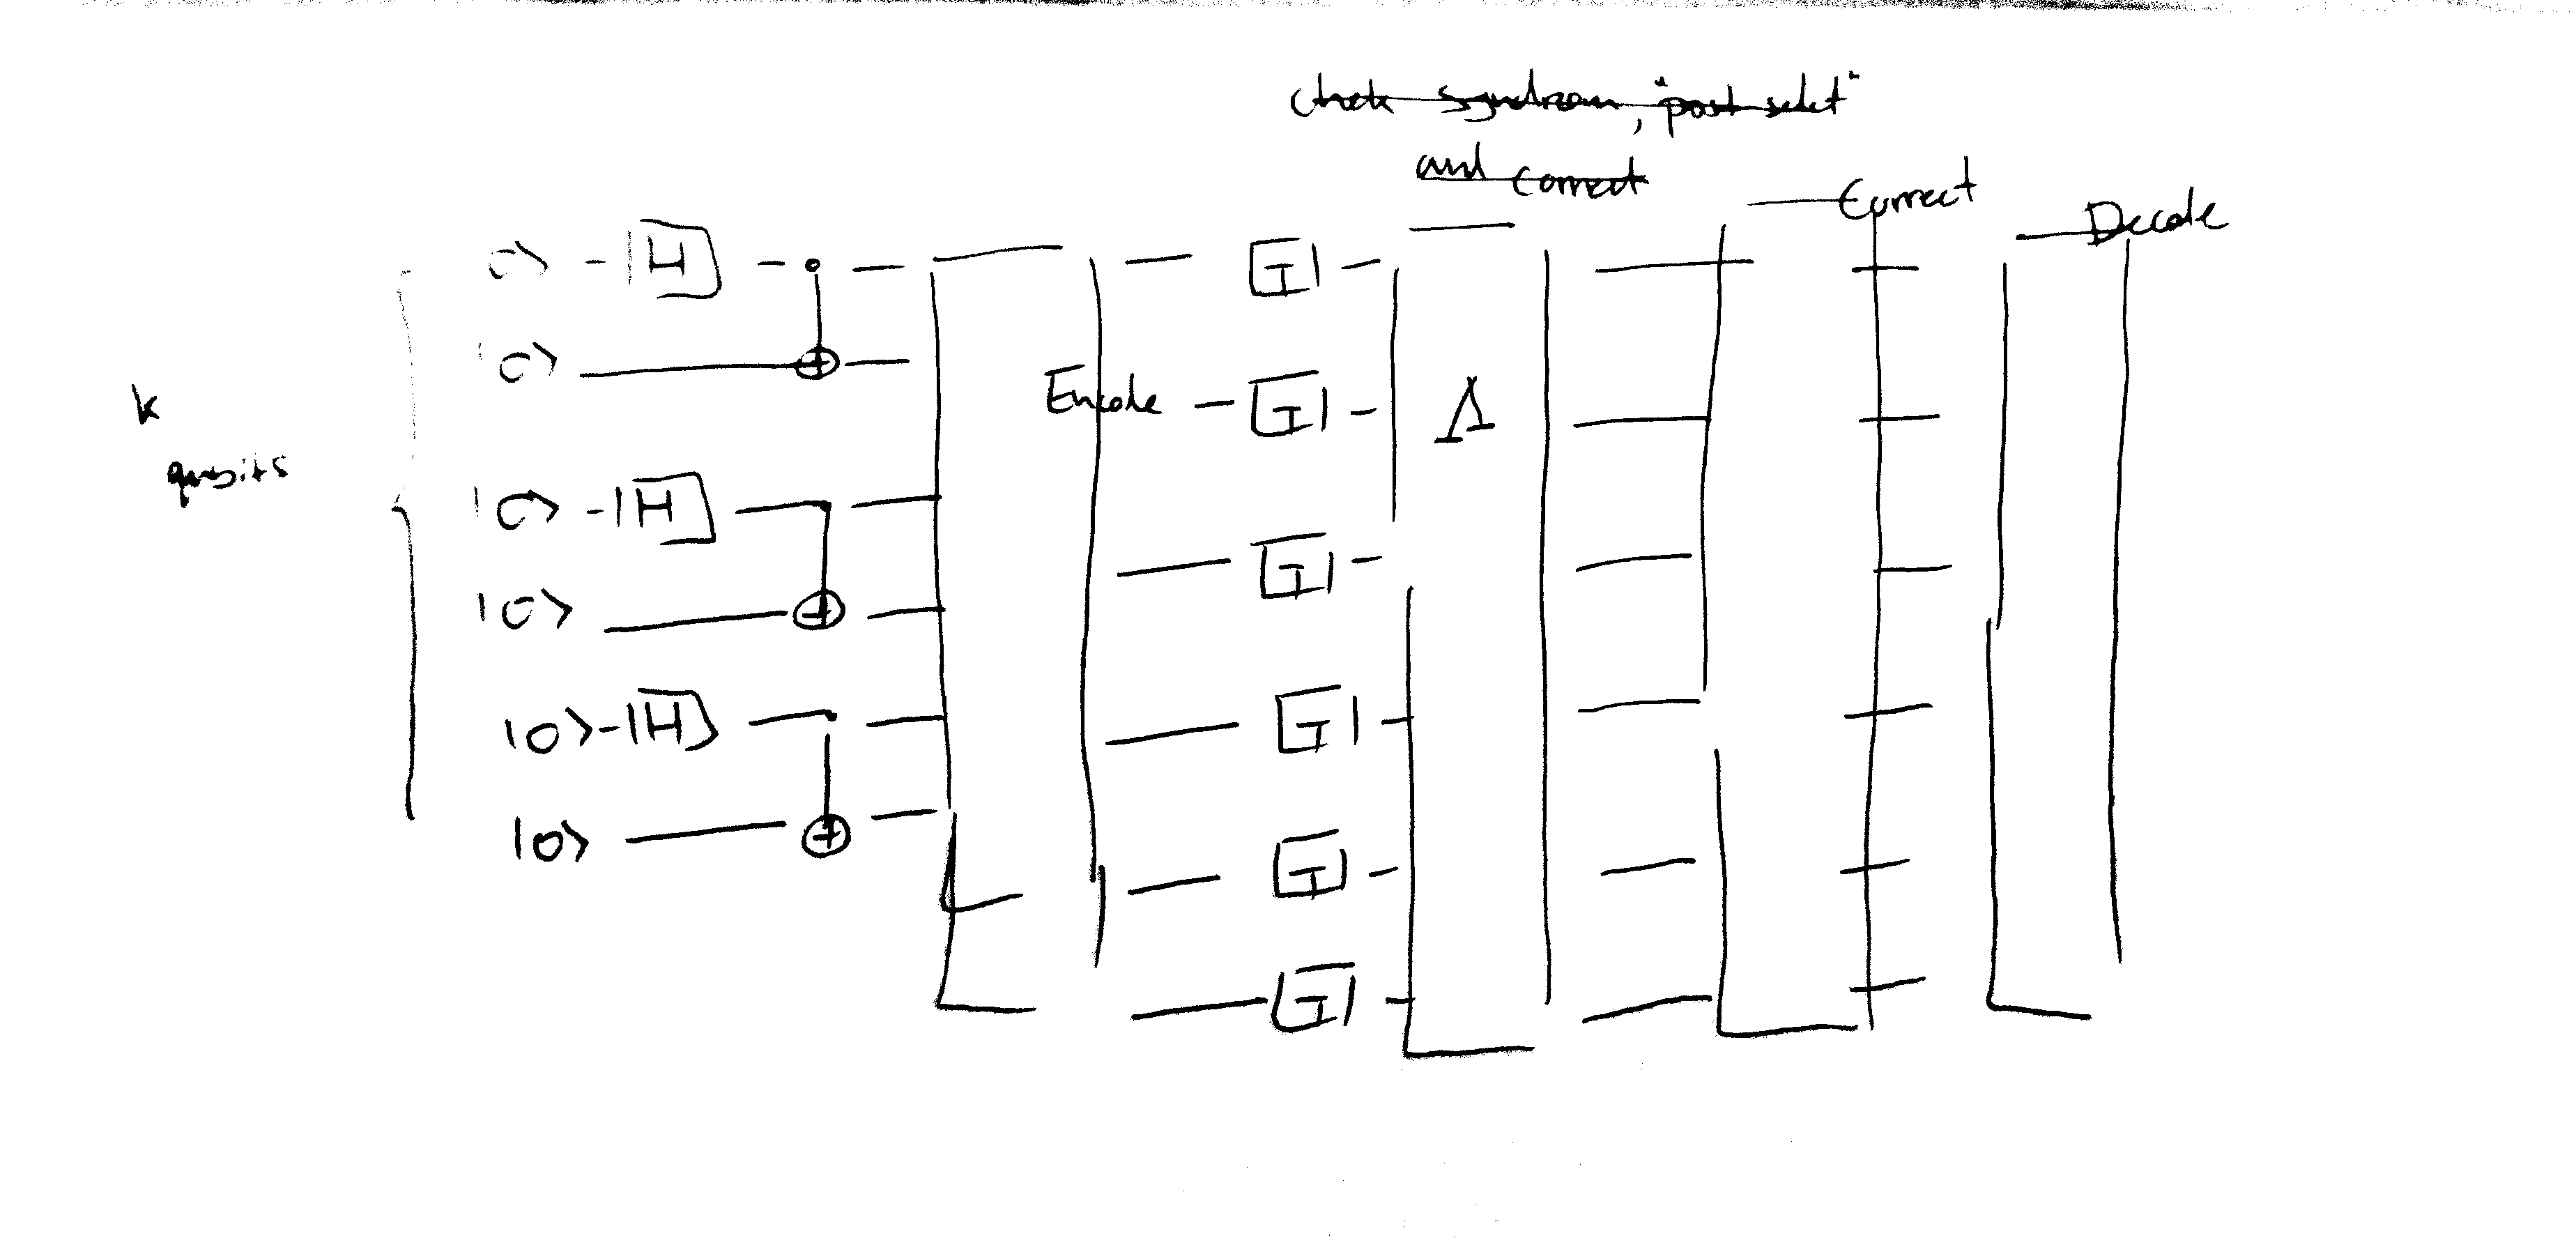
\includegraphics{distil.jpg-out.png}
%}
%  \caption{Quantum Circuit for distillation.}
%  \label{fig:circuit}
%\end{figure}
%
%\begin{claim}
%  \label{claim:phase}
%  The gate $\ket{f} \mapsto \exp \Big(  -  i\pi \sum_{g,h \in G/a}
% X_{g}X_{h}|g\cdot h|  \Big) \ket{f} $ is in the Clifford.
%\end{claim}
%\begin{proof}
%Just decode $f$ and apply \textbf{CZ} between any pair of qubits corresponding
% to the generators $g,h$ such that $g \cap h = 1$. Then encode the state
% again. Observes that \textbf{CZ} is a Clifford gate, and by the fact that the
% code is a CSS code then the decoder and the encoder are both in the Clifford.
%\end{proof}
%Let's denote the circuit defined in \Cref{claim:phase} by $\Lambda$. So we
% have that:
%\begin{equation*}
%  \begin{split}
%    \Lambda^{\dagger}\exp \Big( i\pi/4 \sum_{g} X_{g}|g|  & -  i\pi \sum_{g,h
% \in G/a} X_{g}X_{h}|g\cdot h|  \Big) \ket{f} \\
%= & \exp \Big( i\pi/4 \sum_{g} X_{g}|g|  \Big) \ket{f}
%  \end{split}
%\end{equation*}
%
%Maybe what do we need is to arrange in some way $|g|+|g^{\prime}| = 4k+1$ and
% $\braket{g,f}= \braket{g^{\prime},f^{\prime}}$
%
%
%\begin{claim}
%  For any $m$ codewords $x_{1}..x_{m}$ there is a set of coordinates $I$ and
% $|I| < \alpha n$. Such that:
%  \begin{equation*}
%    \begin{split}
%      \sum_{j \in [n]/I }x_{a}^{j}x_{b}^{j} = 0
%    \end{split}
%  \end{equation*}
%  For any pair $x_{a},x_{b}$.
%\end{claim}
%
%\begin{claim}
%  For any $m$ codewords $x_{1}..x_{m}$ there is a set of coordinates $I$ and
% $|I| < \alpha n$. Such that:
%  \begin{equation*}
%    \begin{split}
%      \sum_{a,b,j \in [n]/I }x_{a}^{j}x_{b}^{j} = 4k
%    \end{split}
%  \end{equation*}
%  For any pair $x_{a},x_{b}$.
%\end{claim}
%

%\paragraph{What about concatination?} So, take a quantum good code. And
% consider a prasintion $k^{\prime}|k|m$ such that $k^{\prime} = \dim
% C_{Z}^{\perp}$ and $k = \dim C_{X}/C_{Z}^{\perp}$. Now concatinate with two
% genorthogonal codes, such that any logical bit of $k$ has wight of 1 module 8
% and the others has weight 0.

\begin{claim}
  Let $C_{A}$ and $C_{A^\prime}$ such that $C_{A^\prime} \subset C_{A}$. Then
  $\left(C_{A}^{\perp} \otimes C_{B}^{\perp}  \right)^{\perp}$, $ C_{A^{\prime}}
  \otimes C_{B^{\prime}}$ form a \textbf{CSS} code $C$ such there exists a
  subspace $V \subset C$ with effictive distance $d$.
\end{claim}

\begin{proof}
  Idea. consider generators of the form $e_{0}\otimes g$. Any codeword  in
  their span is just a first row asssitmentd to a code word of $C_{A}$. If we
  assume less than linear number on that row then we will secucess to decode it,
  $+$ some other generators that we don't care about.
\end{proof}

\begin{equation*}
  \begin{split}
    C_{X} & = \left( \left( C_{A} \otimes C_{0} \right)^{\perp} \otimes
    C_{0}^{\perp}  \right)^{\perp} \\
    C_{Z} & = \left( \left( C_{A} \otimes C_{0} \right) \otimes C_{0}
    \right)^{\perp}
  \end{split}
\end{equation*}

\begin{claim}
  \label{claim:oneg}
  Let $C$ be a code at rate $\rho(C) > 7/8 $ has at least one codeword $x \in
  C$ , such that $|x| =_{8} 1 $.
\end{claim}

\begin{definition}
  We will say that a code $C$ is $(l,m)$-genorthogonal if there exists a
  generator set $G$ for $C$ such that for any $I \subset G$ such that $1 < |I| <
  l$ we have that:
  \begin{equation*}
    \begin{split}
      \sum_{i \in [n]}\prod_{g_{j}\in I \subset G}g_{j}^{i} =_{m} 0
    \end{split}
  \end{equation*}
\end{definition}

\begin{claim} \label{claim:goodgen}
  If there exists a single $(l,m)$-genorthogonal code for a finite length
  $\Delta$, then there is a family of $(l,m)$-genorthogonal good codes.
  Moreover, if there exists a generator in $C_0$ of weight $|\cdot|_m = 1$, then
  there exists a family that also has at least one generator of weight
  $|\cdot|_m = 1$.
\end{claim}
\begin{proof}
  Denote by $C_{0} = \Delta[1,\rho_{0}, \delta_{0}]$ an $(l,m)$-genorthogonal
  code and observes that for any $C = [n,\rho n, \delta n]$ the tensor code
  $C_{0}\otimes C = [\Delta n, \rho_{0} \rho \Delta n, \delta_{0} \delta \Delta
  n]$ is also $(l,m)$-genorthogonal code.

  For the seconed part of the claim, Choose $C$ to be a good code with rate $>
  \left(2^{m}-1\right)/2^{m}$ by \Cref{claim:oneg} there is at least on codeword
  $c$ in $C$ such that $|c| =_{m} 1$.

  So pick the base for $C_{0}\otimes C$ such the first generator is $g_{0}
  \otimes c$ where $g_{0}$ denote a generator of $C_{0}$ satisfies $|g_{0}|
  =_{m} 1$.
  Then $|g_{0} \otimes c | = |g_{0}| \cdot |c| =_{m} 1$.
\end{proof}

\begin{claim}
  Suppose that there exists $(m+1,m)$-genorthogonal code, such that any
  generator of it has weight $| \cdot | =_{m} 1$ then there exists also a family
  of good $(m+1,m)$-genorthogonal codes such that a liner portion of his
  generators $g$ have weight $|g| =_{m} 1$.
\end{claim}

\begin{proof}
  Denote by $C_{0}$ a finte $(m+1,m)$-genorthogonal code, such that any
  generator of it has weight $| \cdot | =_{m} 1$. Let $C$ be a good
  $(m+1,m)$-genorthogonal code with generator $c$ such that $|c| =_{m} 1$, the
  existence of which is given by \Cref{claim:goodgen}. Denote its rate by
  $\rho$. If $C$ has more than $\rho/m \cdot n$ generators at weight $| \cdot |
  =_{m} 1$ then we are done. Otherwise, by the pigeonhole principle, there is an
  $i$ such that more than $\rho/m$ portion of the generators are at weight $
  |\cdot| =_{m} i$. Denote them by $g_{1},g_{2},g_{3}, \dots, g_{m}$.

  Define the set $g_{1}^{^\prime},g_{2}^{\prime}..g_{m}^{\prime}$ as
  \begin{equation*}
    \begin{split}
      g^{\prime}_{t} & = c + \sum_{j=t}^{t+m}g_{j} \\
      & \Rightarrow |g^{\prime}_{t+1}| = |c| + \sum_{t}{ |g_{j}| } +
      \sum_{|I|<l+1}\left|\prod_{g \in I  } \alpha_{\star} g \right| \\
      & =_{m} c + m\cdot i =_{m} c =_{m} 1
    \end{split}
  \end{equation*}
  Now take $C_0 \otimes C$, and set the new generator set to be $g^0_i \otimes
  g'_j$. And it's easy to verify that we got the code we wanted.
\end{proof}

\begin{claim} \label{claim:code}
  There exists, a good LDPC code (classic) $C$ such that $C^{\perp}$ is also a
  good code and a generator set $G$, for exists $G^{\prime} \subset G$ and
  $|G^{\prime}| = \Theta( |G|)$ such:
  \begin{enumerate}
    \item For any pair $x \neq y \in G^{\prime} \rightarrow x\cdot y =_{8} 0$
    \item For any triple $x\neq y,z \in G^{\prime} \rightarrow
      \sum_{i}x_{i}y_{i}z_{i} =_{8} 0$
    \item For any $x \in G^{\prime} \rightarrow |x| =_{8} 1$
  \end{enumerate}
\end{claim}

\begin{claim}
  There is $n \rightarrow \Theta(n)$ magic states distillation into a binary
  qldpc code with $\Theta(\sqrt{n})$ distance, and therefore with asymptotic
  overhead approaching $1$
\end{claim}

\begin{proof}
  For the encoding we are going to use the hyperproduct code defined in
  \cite{Tillich_2014}. Let $C$ be the code given by \Cref{claim:code} and
  consider the hyperproduct of $C$ with itself $Q = Q(C \times_{H} C)$. In
  addition, denote by $C_{X},C_{Z}$ the CSS representation of $Q$.

  By the fact that $C^\perp$ is also a good code, then $Q$ is a positive rate,
  square root distance code. Let $\rho$ be the rate of $C$ and $1 - \rho$ be the
  rate of $C^{\perp}$. As $\rho > 0$, then one can find $I \subset [n]$
  coordinates such that for any $i \in I$ the indicator $e_{i} \not\in
  C^{\perp}$. Hence, it holds from \cite{Tillich_2014} that any vector of the
  form $e_{i}\otimes x$ is a codeword of $C_{X}/C_{Z}^{\perp}$.

  Denote by $\rho^{\prime}$ the portion of $G^{\prime}$ as defined in
  \Cref{claim:code}, and define $S$ to be:
  \begin{equation*}
    \begin{split}
      S = \left\{ e_{i} \otimes x| e_{i} \not\in C^{\perp}, x \in G^{\prime}
      \right\}
    \end{split}
  \end{equation*}
  Observes that $|S| = \rho^{\prime}\rho n^{2}$ and in addition $S$ satisfies
  the properties in \Cref{claim:code}. Denote by $f$ a codeword supported only
  on $S$ and denote by $X_{s}$ the indecator that indicate that $s$ supports
  $f$. Thus:
  \begin{equation*}
    \begin{split}
      T^{\otimes n}\ket{f}  = \exp \Big( i\pi/4 & \sum_{g} X_{g}
        \overbrace{|g|}^{8k+1}  \\
        & -  2 \cdot i \pi/4  \overbrace{\sum_{g,h} X_{g}X_{h}|g\cdot h|}^{8k}
        \\
        & +  4 \cdot i\pi/4 \overbrace{ \sum_{g,h} X_{g}X_{h}X_{l}|g\cdot h
          \cdot
      l| }^{8k } \Big) \ket{f} \\
      & \\
      =   \exp \Big( i\pi/4 & \sum_{g \in S} X_{g} \Big) \ket{f}
    \end{split}
  \end{equation*}
  Therefore we can, generate the enocded (\ctt{For now without spanning on on
  $C_{Z }^{\perp}$} ) product of $T^{\otimes|S|}\ket{+}^{|S|}$:
  \begin{equation*}
    \begin{split}
      \prod_{s \in S} \Big( \ket{0} + \exp \left( i\pi/4 \right) \ket{s} \Big)
    \end{split}
  \end{equation*}

  \ctt{What is left:
    \begin{enumerate}
      \item Show that one can generate $ \prod_{s \in S} \Big(
          \ket{C_{Z}^{\perp}} + \exp \left( i\pi/4 \right) \ket{C_{Z}^{\perp} +
          s}
        \Big)$ without propagate the errors. I think I know how to do it.
      \item Compute a threshold $p_{0}$ for using Baravi construction.
    \end{enumerate}
  }

  Thus we have that $\gamma = \log(n/k)/\log(d) =
  \log(n/|S|)/\log(\Theta(\sqrt{n})) \rightarrow 0$ and the overhead growes as
  $\log^{\gamma}(n) \rightarrow 1$ \cite{bravyi2012magic},
  \cite{meier2012magicstate}.
\end{proof}

\cite{leverrier2022quantum}
\cite{moore1998parallel}
\cite{bravyi2012magic}
\cite{Tillich_2014}
\cite{meier2012magicstate}


% Triorthogonal

\fi



%\cite{leverrier2022quantum}
%\cite{moore1998parallel}
%\cite{Tillich_2014}
%\cite{meier2012magicstate}
%\cite{bravyi2012magic}
\printbibliography

\end{document}

